\documentclass{ttp}

%--------------------------------------------- Basic packages (could be expanded by author)%
\usepackage{floatrow}
%\usepackage{graphicx,wrapfigure}
\usepackage{graphicx}
\usepackage[intlimits]{amsmath}
\usepackage{amssymb}
\usepackage{exscale}
\usepackage{hyperref}
\usepackage{times}
%\usepackage{xparse}
\usepackage{fontspec}
%\ifdefined\directlua
%  \usepackage{fontspec}
%\else
%  \usepackage[T1]{fontenc}
%  \usepackage[nomath]{lmodern}
%\fi
%Для пришвидшення компіляції закоментив \usepackage{subfigure}
%\usepackage{subfigure}
%\usepackage{fontspec-patches}	
	% <-- DO NOT REMOVE this package,
				%       because the fonts (Times New Roman and Arial) will not be used in the document.
					% 	   If you don`t have this package, you can get it from the Internet or you can get this
					%       package from the archive The_Fontspec_package.zip which you downloaded with
					%       this current file.

%---------------------------------------------If you need include the .eps files, please uncomment the package bellow.%
%\usepackage{epsfig}

%--------------------------------------------- Override fonts to Times New Roman and Arial%
\renewcommand{\large}{\fontsize{14}{18pt}\selectfont}
\renewcommand{\small}{\fontsize{11}{13.6pt}\selectfont}
\setmainfont{Times New Roman}
\setsansfont{Arial}

%--------------------------------------------- New commands for quick editing of the document%
\newcommand{\titleformat}{\sffamily\bfseries \large}						%	<--- Doc. title
\newcommand{\authorformat}{\sffamily \large}							%	<--- Authors
\newcommand{\keywordsformat}{\noindent \small \sffamily}				%	<--- Kyewords
\newcommand{\abstractformat}{\noindent \textbf}						%	<--- Abstract
\newcommand{\contentformat}{\rmfamily \normalsize\vspace{18pt}}			%	<--- Main content
\newcommand{\email}{\sffamily \small \vspace{-8pt}}						%	<--- E-mail
\renewcommand{\subsection}{\textbf}	

%--------------------------------------------- Make all internal and external links - black color%
\hypersetup{
    colorlinks,%
    citecolor=black,%
    filecolor=black,%
    linkcolor=black,%
    urlcolor=black
}

%--------------------------------------------- Set the basic parameters of the page. DO NOT CHANGE!%
\special{papersize=210mm,297mm}
\textheight=25.6cm

%--------------------------------------------- For the Publisher to Enter:

\begin{document}

\title{\titleformat Variability in FeB Pair Association Rates in Silicon under Ultrasound Loading: Effects of Acoustic Wave Types}

%\author{ FULL First Author \inst{1}$^{,\rm{a}}$ \textbf{,} FULL Second Author \inst{2}$^{,\rm{b}}$ and Last Author \inst{3}$^{,\rm{c}}$}
\author{\authorformat OLIKH Oleg \inst{1}$^{,\rm{a}}$ and ARUTYUNOV Nikolay \inst{,2,3}$^{,\rm{b}}$}

\institute{\sffamily Department of General Physics, Taras Shevchenko National University of Kyiv, Kyiv, Ukraine
\and Department of Physics, Martin Luther University Halle, Halle, Germany
\and Leibniz-lnstitut für Kristallzüchtung (IKZ), Berlin, Germany}

\maketitle

\begin{center}
\email{ $^{\rm a}$olegolikh@knu.ua, $^{\rm b}$n\_arutyunov@yahoo.com}
%\email{ $^{\rm a}$olegolikh@knu.ua, $^{\rm b}$n_arutyunov@yahoo.com}
\end{center}


\keywordsformat{{\textbf{Keywords:}}  Ultrasound, Silicon, Iron-boron pair, Point defect, Acousto-defect interaction, Positron annihilation
spectroscopy.}

\contentformat

\abstractformat{Abstract.}
Initially, this work briefly outlines how ultrasound can modify and characterize the defect system in semiconductors.
Then, the study experimentally examines the effect of different types of acoustic waves on the association
of FeB pairs in monocrystalline silicon.
The results reveal that as the frequency of longitudinal waves increases, the ultrasound's effectiveness in accelerating the association rate decreases.
Conversely, exciting transverse waves show the opposite trend.
The study also assesses the potential to obtain a positron-annihilation response from the FeB complex in silicon,
highlighting the advantages of conducting such measurements under ultrasound loading of the crystal.


\section{Introduction}\label{S1}
\vspace{-6pt}

Defects are well known to impact the properties of semiconductor devices significantly.
In this regard, defect engineering, which involves controlled tuning of the defect-impurity subsystem to achieve new crystal, structure, or device properties, is crucial.
One of the powerful tools for such active defect engineering is applying acoustic vibrations in the ultrasonic frequency range.
For example, ultrasound treatment can stimulate the diffusion of various defects at temperatures close to room temperature
due to the acoustically induced (AI) decrease in activation energy or over-barrier motion
\cite{Ostapenko1999,
%Ostap:PhotoLum ?,
BORKOVSKA2003}.
Additionally, ultrasound (US) can cause the reconstruction of intrinsic point defects \cite{Bahar2003, RITTER2008, Wosinski}
or the annealing of radiation-induced defects
\cite{UST:OstrovCsI,
UST:LED_SM,
GORB2020,
Gorb2010}.
Often, ultrasound serves not as the primary tool for modification
but as an additional factor influencing the process during conventional technological operations,
such as ion implantation \cite{Litovchenko2015, ROMANJUK2005MatSci} or film deposition \cite{Wang:JLum, US:ZnOfilm}.

In addition to the residual effects of ultrasound, acousto-dynamic effects also attract significant interest.
In this case, changes in the state of defects and modifications to semiconductor properties
are observed only under ultrasound loading (USL) conditions.
After the cessation of acoustic wave (AW) propagation,
the defect subsystem returns to its initial state, and the properties revert to their original condition.
In particular, acousto-induced effects have been discovered, including changes in the configuration of metastable defects
(FeB pairs and A-centers in Si \cite{YOlikhTPL2011, Ostrovskii2001},
EL2 in GaAs \cite{buyanova1994}, DX in AlGaAs \cite{belyaev1994}),
recharging of point defects
(Te, vacancy, V-O in silicon structures \cite{Korotchenkov1995, Olikh2018JAP, Olikh:Ultras},
heterostructures GaAs/AlGaAs \cite{Zaveryukhin2002}),
reconstruction of the Cottrell cloud
(SiGe/Si, CdTe:Cl, CdHgTe \cite{Kuryliuk2009,
%(або залишити Ostrovskii2001),
YOlikh:SupMicr, Vlasenko2000}),
and the formation of non-equilibrium dislocation clusters
(GaP \cite{Gontaruk1998}).
Such effects enable the creation of functional electronic devices,
where control of the information signal relies on the inhomogeneities in the medium, which arise from the US action.


Acoustic waves also serve as a tool for characterizing the defect subsystem of semiconductors.
For example, modifying elastic moduli during the formation of Jahn-Teller defects can cause extrema to appear in the temperature dependencies of US velocity and absorption.
Such anomalies enable the successful investigation of intrinsic defects \cite{USM:Mitsumoto2014, USM:SEYIDOV2016}
and substitutional atoms \cite{USM:Zhevstovskikh, USM:YI2009} across various crystals.
Another approach to US modification of traditional defect research methods involves acousto-dynamic effects.
Specifically, while ultrasound propagates, the system's response to external influences unrelated to elastic vibrations changes.
It allows for obtaining more detailed information about defects than without AW.
In particular, defect identification has been carried out using modified DLTS spectra,
transmission and reflection measurements \cite{Kor1996, Ostrovskii2001, OSTROVSKII2000, SST:USmethod}.

This work examines the potential advantages of the acousto-positron perturbation technique,
which involves conducting positron annihilation spectroscopy (PAS) under ultrasonic loading.
The previously mentioned possible AI changes in the state of defects indicate that ultrasound can modulate the conventional PAS signal,
including both positron annihilation lifetime spectroscopy (PALS) and coincidence Doppler broadening (CDB) spectroscopy
(encompassing both high-momentum component $W$ and low-momentum component $S$ --- see, e.g. \cite{Krause1999}).
Consequently, such studies could be more informative and, more importantly, may enhance the method's capabilities.
For example, PAS is known to be most suitable for studying negatively charged and neutral vacancy-type defects \cite{Makkonen2024,Tuomisto2013}.
The advantages of ultrasound as a defect engineering tool \cite{Olikh2018JAP} may enable the expansion
of the class of defects that can be studied using positron annihilation.
In other words, the combination of PAS and ultrasound can provide new opportunities for studying defects in semiconductors,
and this work aims to discuss the possibilities and prospects of this approach.

This study is focused on iron-related defects in Si:B.
Iron is known to be one of the most detrimental metallic impurities in photovoltaic silicon.
In $p$-type Si, iron atoms are predominantly bound into $\mathrm{Fe}_i^+\mathrm{B}_s^−$ pairs
or occupy interstitial sites as $\mathrm{Fe}_i^+$.
%forming defects that are traditionally difficult to study using PAS.
The subsequent section presents experimental results that illustrate the variability in the effect of ultrasound on the defect subsystem.
Specifically, it examines how vibrations with varying types influence the AI transformation processes
between Fe$_i$ and FeB, which can occur readily at room temperature \cite{FeBAssJAP2014}.
The penultimate section is devoted to quantitative estimates of positron annihilation in the FeB complex.
Finally, the article concludes in the last section.



\section{Peculiarities of FeB Pair Association under Ultrasonic Loading Condition}

\noindent \textbf{Experiment details.}
The $n^+$-$p$-$p^+$-Si samples were used in the experiment.
The structure was fabricated from a 380~$\mu$m thick single-crystal
$p$-type Cz-Si:B [100] wafer
with the resistivity of about 10~$\Omega\cdot$cm.
The $n^+$ emitter (sheet resistance of $20-30$~$\Omega/\Box$,
thickness of $0.7$~$\mu$m) and $p^+$ back surface field layer ($10-20$~$\Omega/\Box$, $0.6$~$\mu$m) were formed by diffusion from the gas phase.
On the front surface, the antireflective and passivating SiO$_2$ (40~nm) and Si$_3$N$_4$ (30~nm) layers
were formed.
The solid and grid Al contacts were formed by magnetron sputtering on the back and front surfaces, respectively.
The area of the samples used in the experiment was $1.52\times1.535$~cm$^2$.
The iron impurity concentration [Fe] in the solar cell base varied from $2\times10^{11}$ to $5\times10^{13}$~cm$^{-3}$ for different samples.

The study examines the characteristic association time of FeB pairs $\tau_\mathrm{ass}$ under conditions with and without ultrasound loading.
The $\tau_\mathrm{ass}$ was determined by analyzing the recovery kinetics of the  short-circuit current under monochromatic lighting
after  the light-induced dissociation of FeB pairs, using methodology \cite{Olikh2021JAP, Olikh2022:JMatSci}.

In the case of USL, the AWs were applied to the samples in the [100] direction using a LiNbO$_3$ piezoelectric transducer.
The USL experiments were designed with careful control over the following experimental parameters:
1)~the type of excited waves: either transverse or longitudinal waves were utilized;
2)~acoustic wave frequency: $f_\mathrm{US}$ was varied between 2 and 30 MHz;
3)~US intensity: $W_\mathrm{US}$ was adjusted up to a maximum of 2.0~W/cm$^2$;
4)~measurement temperature: the experiments were performed between 300 and 340 K.
We shielded the transducer to avoid the effects of the piezoelectric field.
For more details on ultrasound excitation, please refer to \cite{Olikh2021JAP, Olikh2022:JMatSci}.

\noindent \textbf{Results of Acousto-induced Changes in Fe Ion Migration.}
The experiments revealed that the AWs presence leads to an increase in the association rate of FeB pairs.
As shown in Fig.~\ref{fig1}, the characteristic association time of FeB pairs
under ultrasound loading, $\tau_\mathrm{ass}^\mathrm{US}$,
exhibits a decrease compared to the value $\tau_\mathrm{ass}^0$ obtained in the USL absence.
It was reported that $\tau_{ass}$ depends on the boron concentration $N_A$
and temperature \cite{FeBAssJAP2014}:
\begin{equation}
\label{eqTass}
\tau_{ass}=\frac{5.7\times10^5T}{N_A}\exp\left(\frac{E_m}{kT}\right)\,,
\end{equation}
where
$E_m$ is the energy of Fe$_i$ migration.
Therefore, the observed AI decrease in $\tau_\mathrm{ass}$ implies a lowering migration energy:

\thisfloatsetup{capposition=beside,%
      capbesideposition={right,top},
      capbesidewidth= 0.5\textwidth,
      floatwidth= 0.45\linewidth
  }

\begin{figure}
	\centering
%     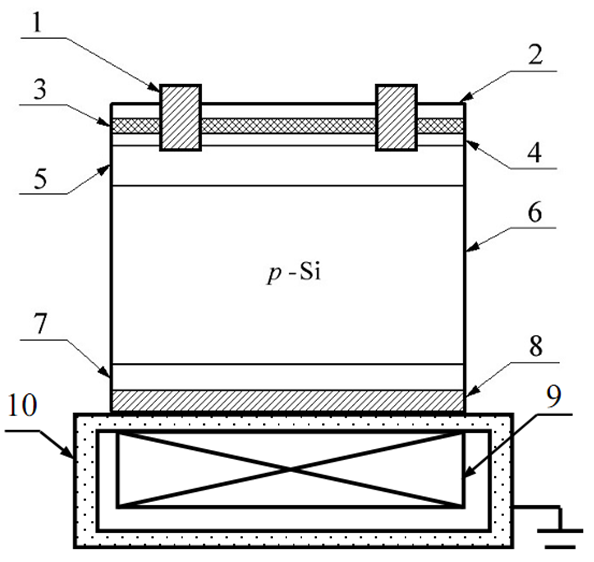
\includegraphics[width=0.45\linewidth]{Fig1.png}
     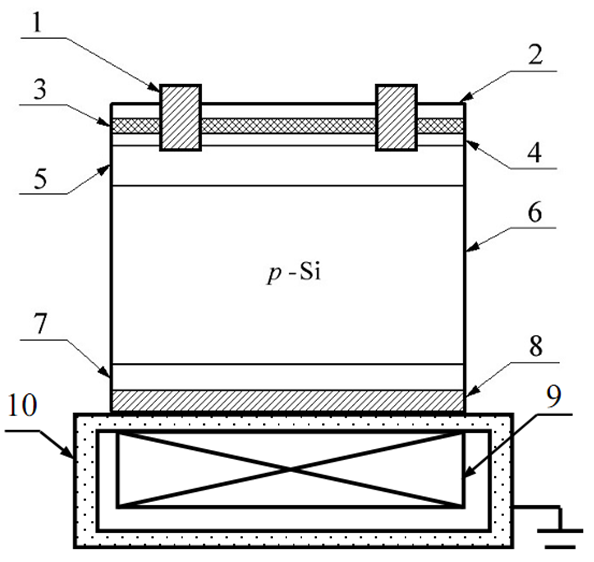
\includegraphics[width=\linewidth]{Fig1.png}
	  \caption{Measured short circuit current plotted as a function of the time after FeB decay
      without USL (1, 3, 5, empty black marks) and under USL (2, 4, 6. filled red marks).
      $T$, K: 300 (1, 2), 320 (3, 4), 340 (5, 6).
      The values of $\tau_\mathrm{ass}^0$ and $\tau_\mathrm{ass}^\mathrm{US}$ obtained
      by the methodology described in \cite{Olikh2021JAP,Olikh2022:JMatSci} are shown also.
      [Fe]=$1.9\times10^{13}$~cm$^{-3}$.
}\label{fig1}
\end{figure}

\begin{equation}
\label{eqEmUs}
E_m \xrightarrow{\mathrm{US}} E_{m,0}-\Delta E_\mathrm{US}\,,
\end{equation}
where
$E_{m,0}$ denotes the migration energy in the USL absence,
as previously reported in \cite{FeBAssJAP2014}
and independently estimated by us through measurements performed in the no-USL configuration
$E_{m,0}\cong(0.655\pm0.002)$~eV;
$\Delta E_\mathrm{US}$ is the AI change in migration energy.
In fact, the value of $\Delta E_\mathrm{US}$ serves as a quantitative measure
of the US influence, and we will focus on examining its relationships with various factors in the following analysis.
It is worth noting that the influence of longitudinal AWs on the $E_m$ value,
its distinct features, and some speculative ideas regarding its underlying mechanism have been reported previously \cite{Olikh2021JAP,Olikh2022:JMatSci}.
This work seeks to elucidate the differences in AI effects when waves of varying types are generated.

Firstly, we note that the magnitude of the AI effect exhibits negligible dependence
on iron concentration, regardless of whether longitudinal or transverse waves are excited.
As illustrated in Fig.~\ref{fig2}, the values of $\Delta E_\mathrm{US}$ exhibit a high degree of similarity
in magnitude for samples with distinct [Fe] values under the same experimental conditions
(temperature, US intensity, and frequency).
Thus, regardless of the nature of lattice atom displacement,
the AI effect is primarily determined by the interaction between the AW and isolated defect
rather than by the collective behavior of defects.

\begin{figure}
	\centering
     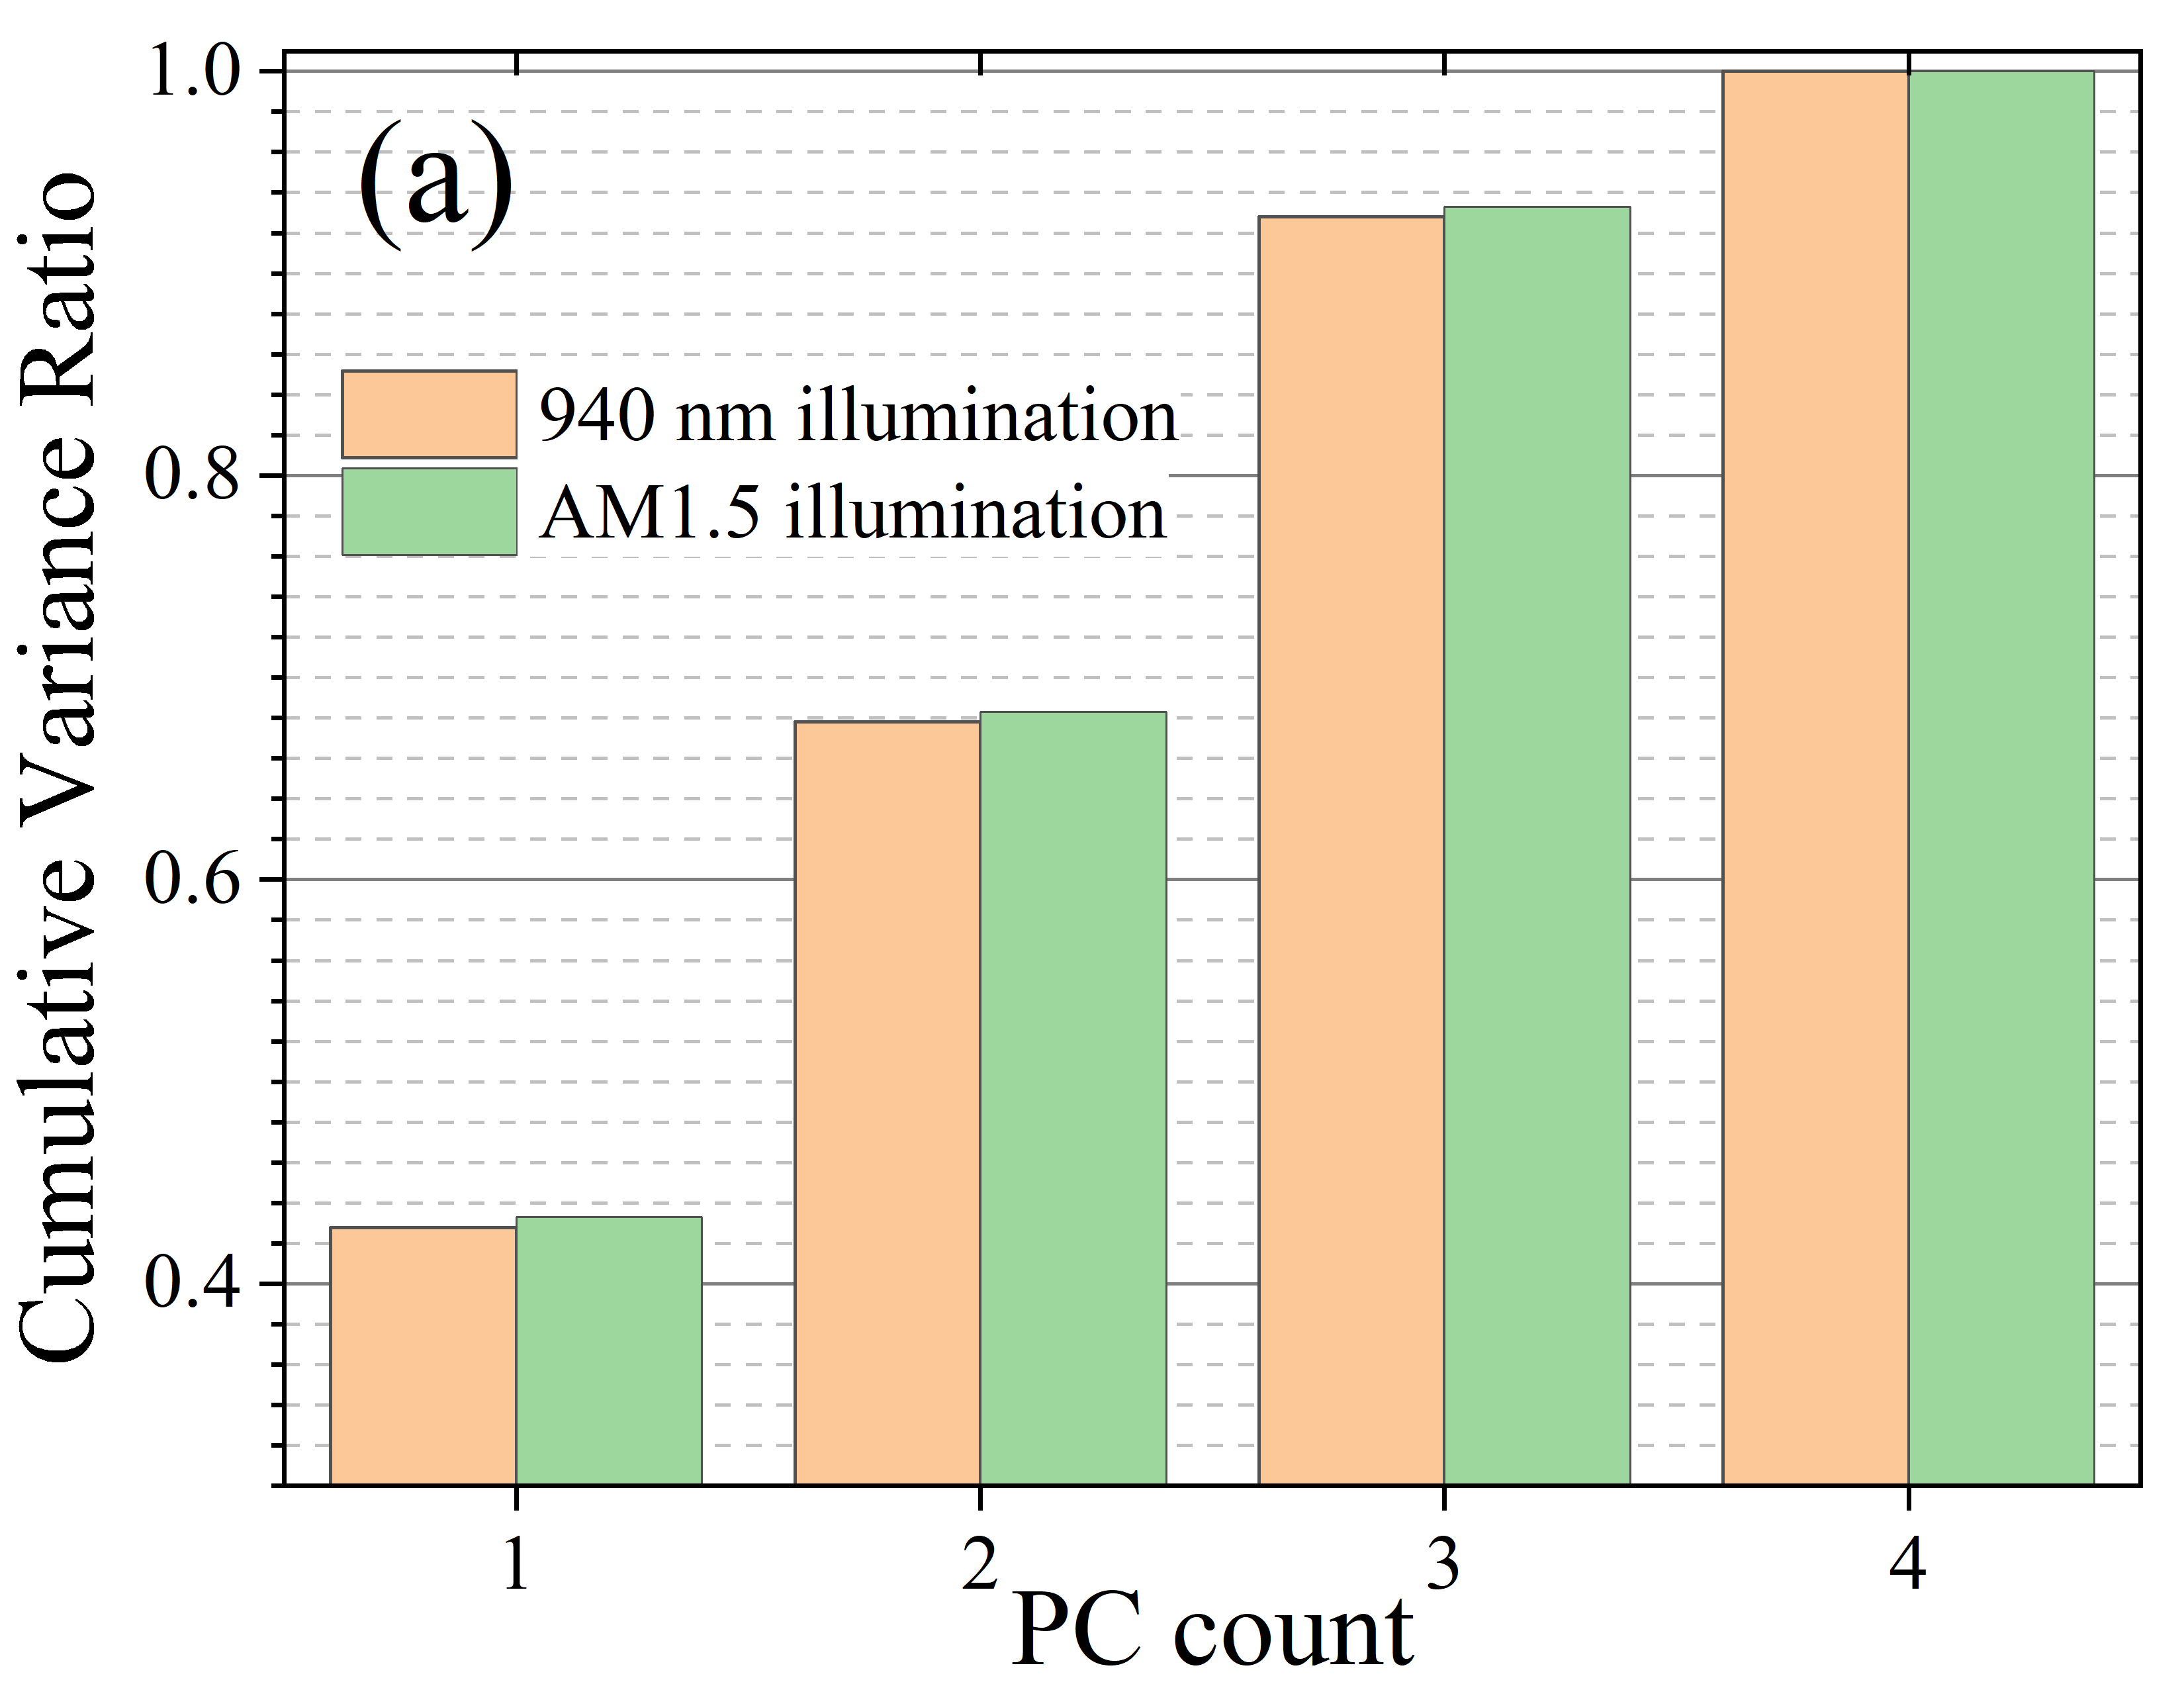
\includegraphics[width=0.4\linewidth]{Fig2a.png}
     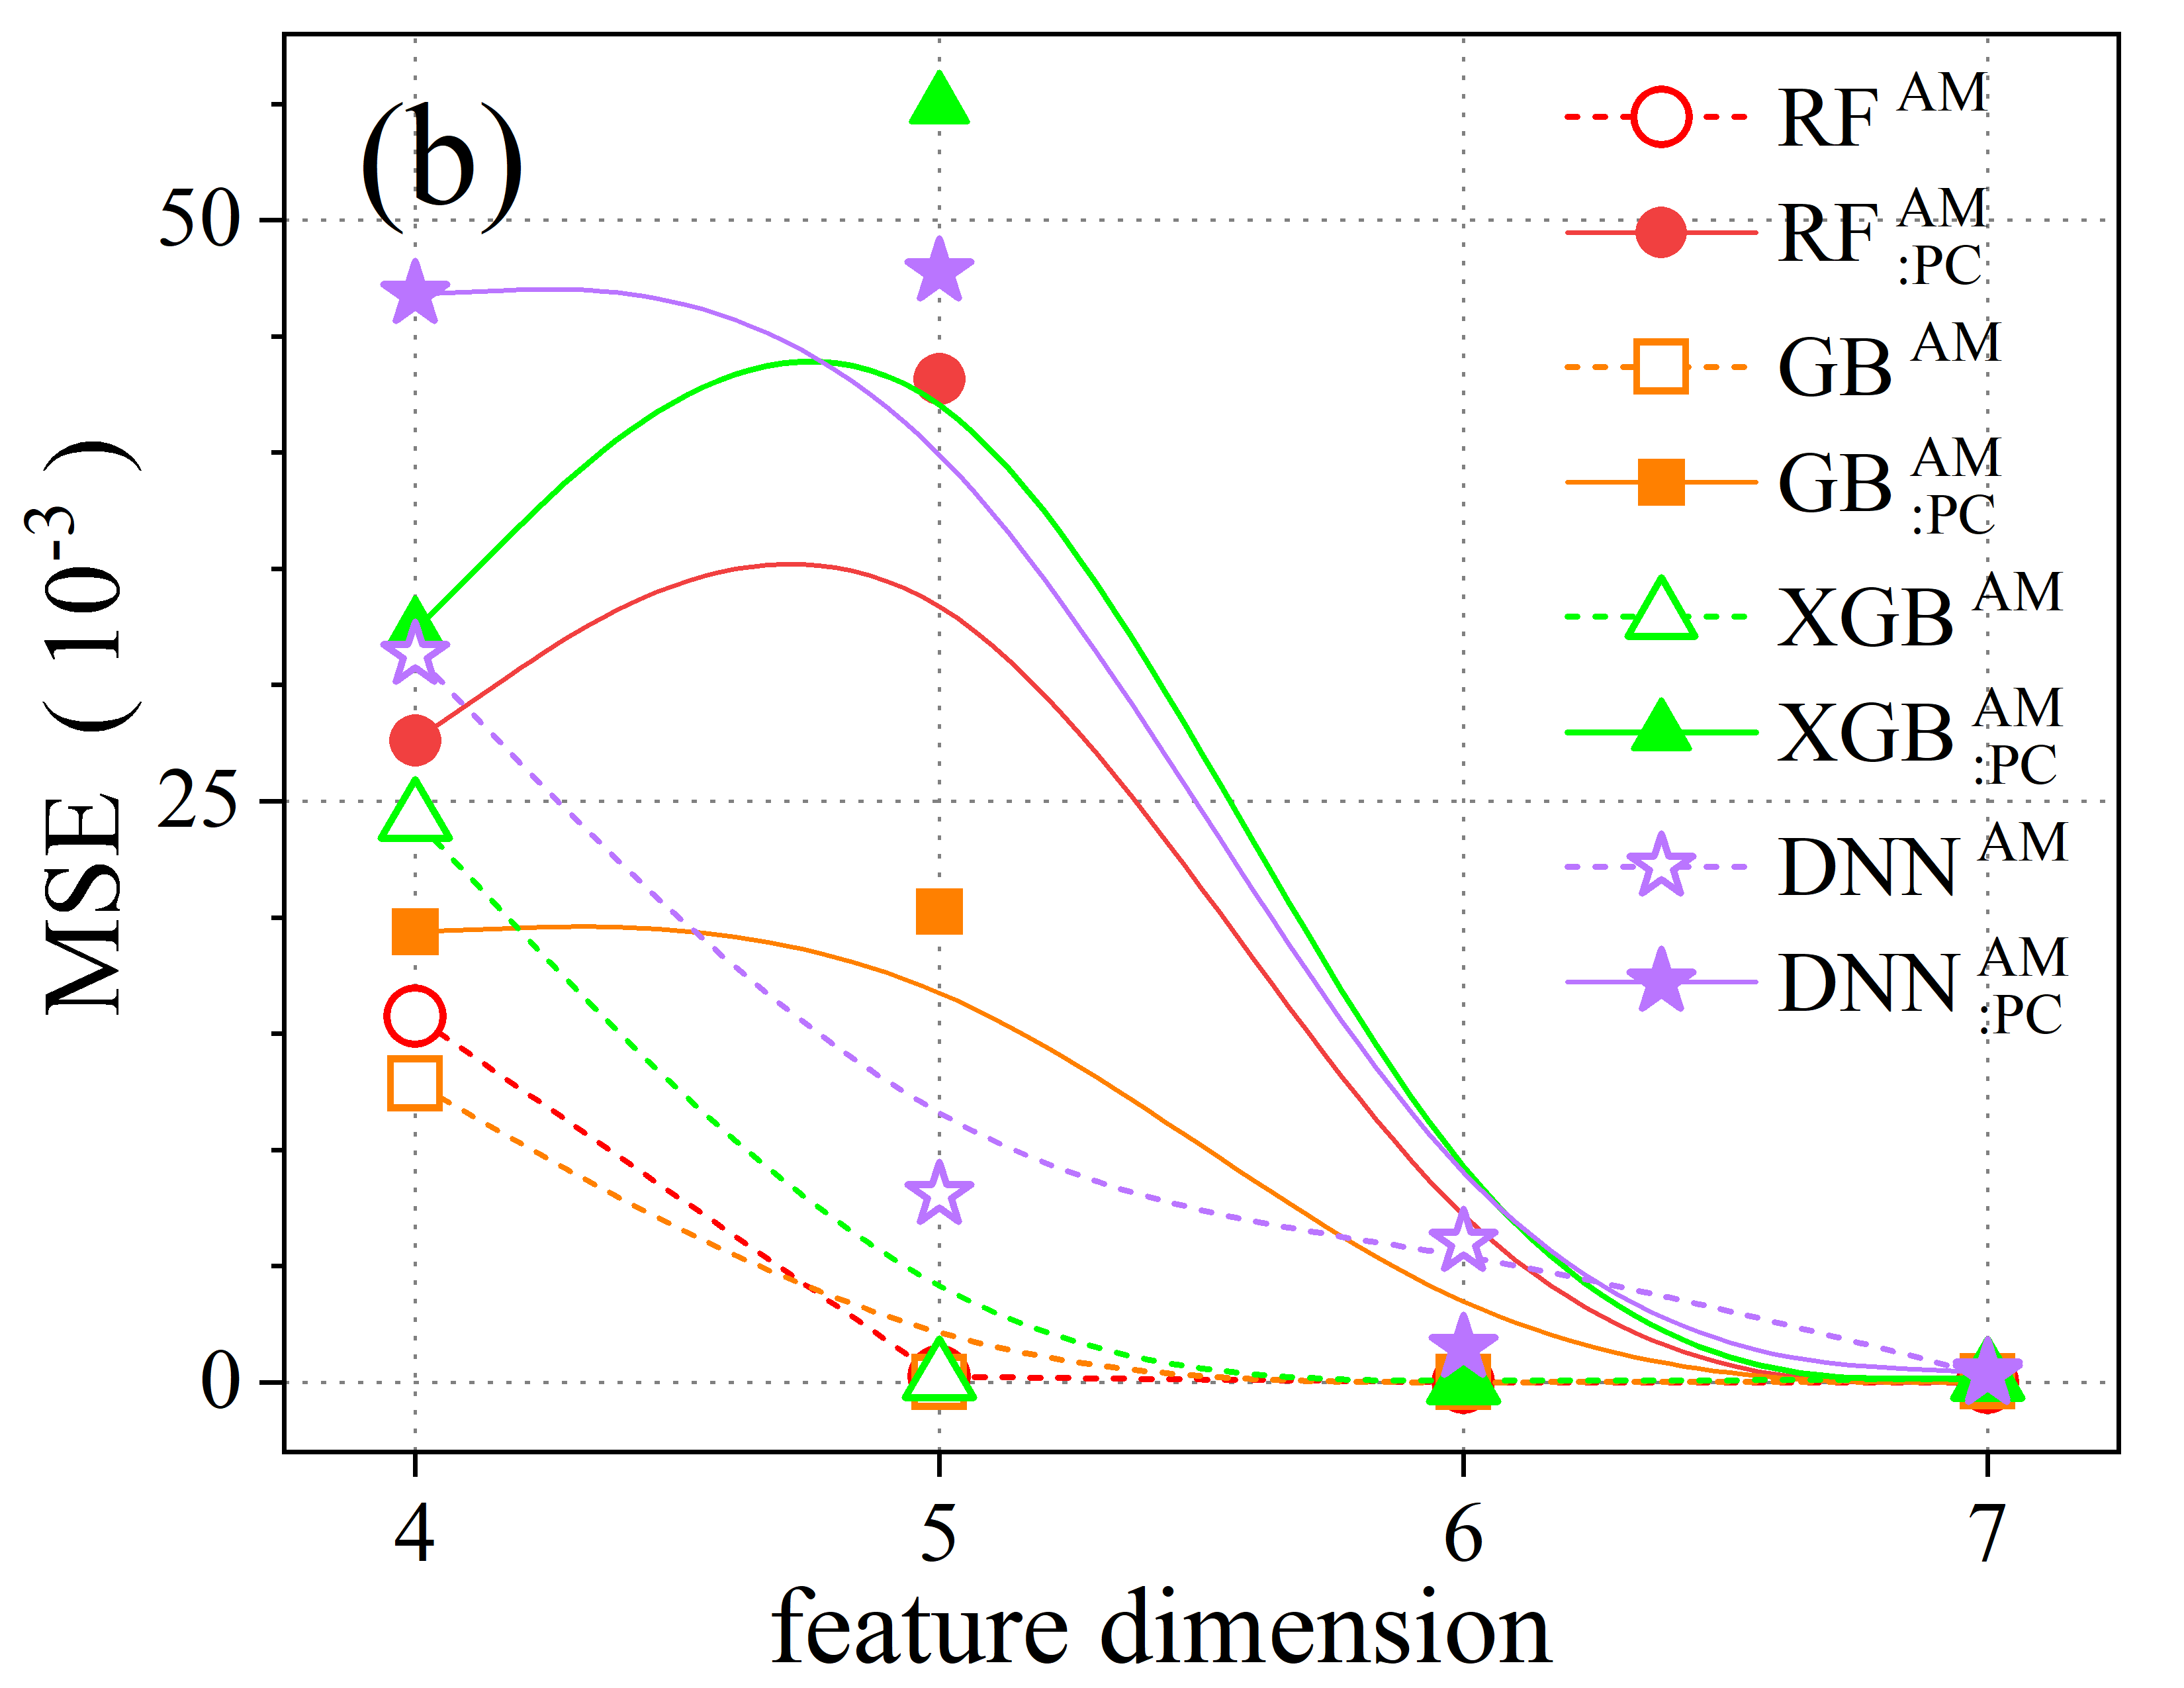
\includegraphics[width=0.4\linewidth]{Fig2b.png}
	  \caption{Dependencies of AI change in migration energy on US intensity for
       samples with different  iron concentrations.
       $f_\mathrm{US}$, MHz: 5.40 (a), 5.23 (b).
       AW type: longitudinal (a), transverse (b).
       $T=340$~K.
}\label{fig2}
\end{figure}

As shown in Fig.~\ref{fig2}, at a frequency of 5~MHz,
the $\Delta E_\mathrm{US}$ values exhibit a linear dependence on US intensity,
holding for both longitudinal and transverse wave excitations.
A similar trend is also observed at other frequencies --- see Fig.~\ref{fig3}.
As a result, the intensity dependence of the AI effect at constant temperature can be expressed as follows:
\begin{equation}\label{eq3O}
  \Delta E_\mathrm{US}(W_\mathrm{US})@ T = \beta_\mathrm{US} W_\mathrm{US}\,,
\end{equation}
where
the intensity coefficient $\beta$ represents the effectiveness of the US effect
in converting the energy of elastic vibration into a modification of the migration energy.
The presented data reveal that $\beta$ exhibits a decreasing trend
with increasing frequency when longitudinal waves are employed (Fig.~\ref{fig3}a).
In contrast, an opposite frequency dependence is observed when transverse waves are excited (Fig.~\ref{fig3}b).

\begin{figure}
	\centering
     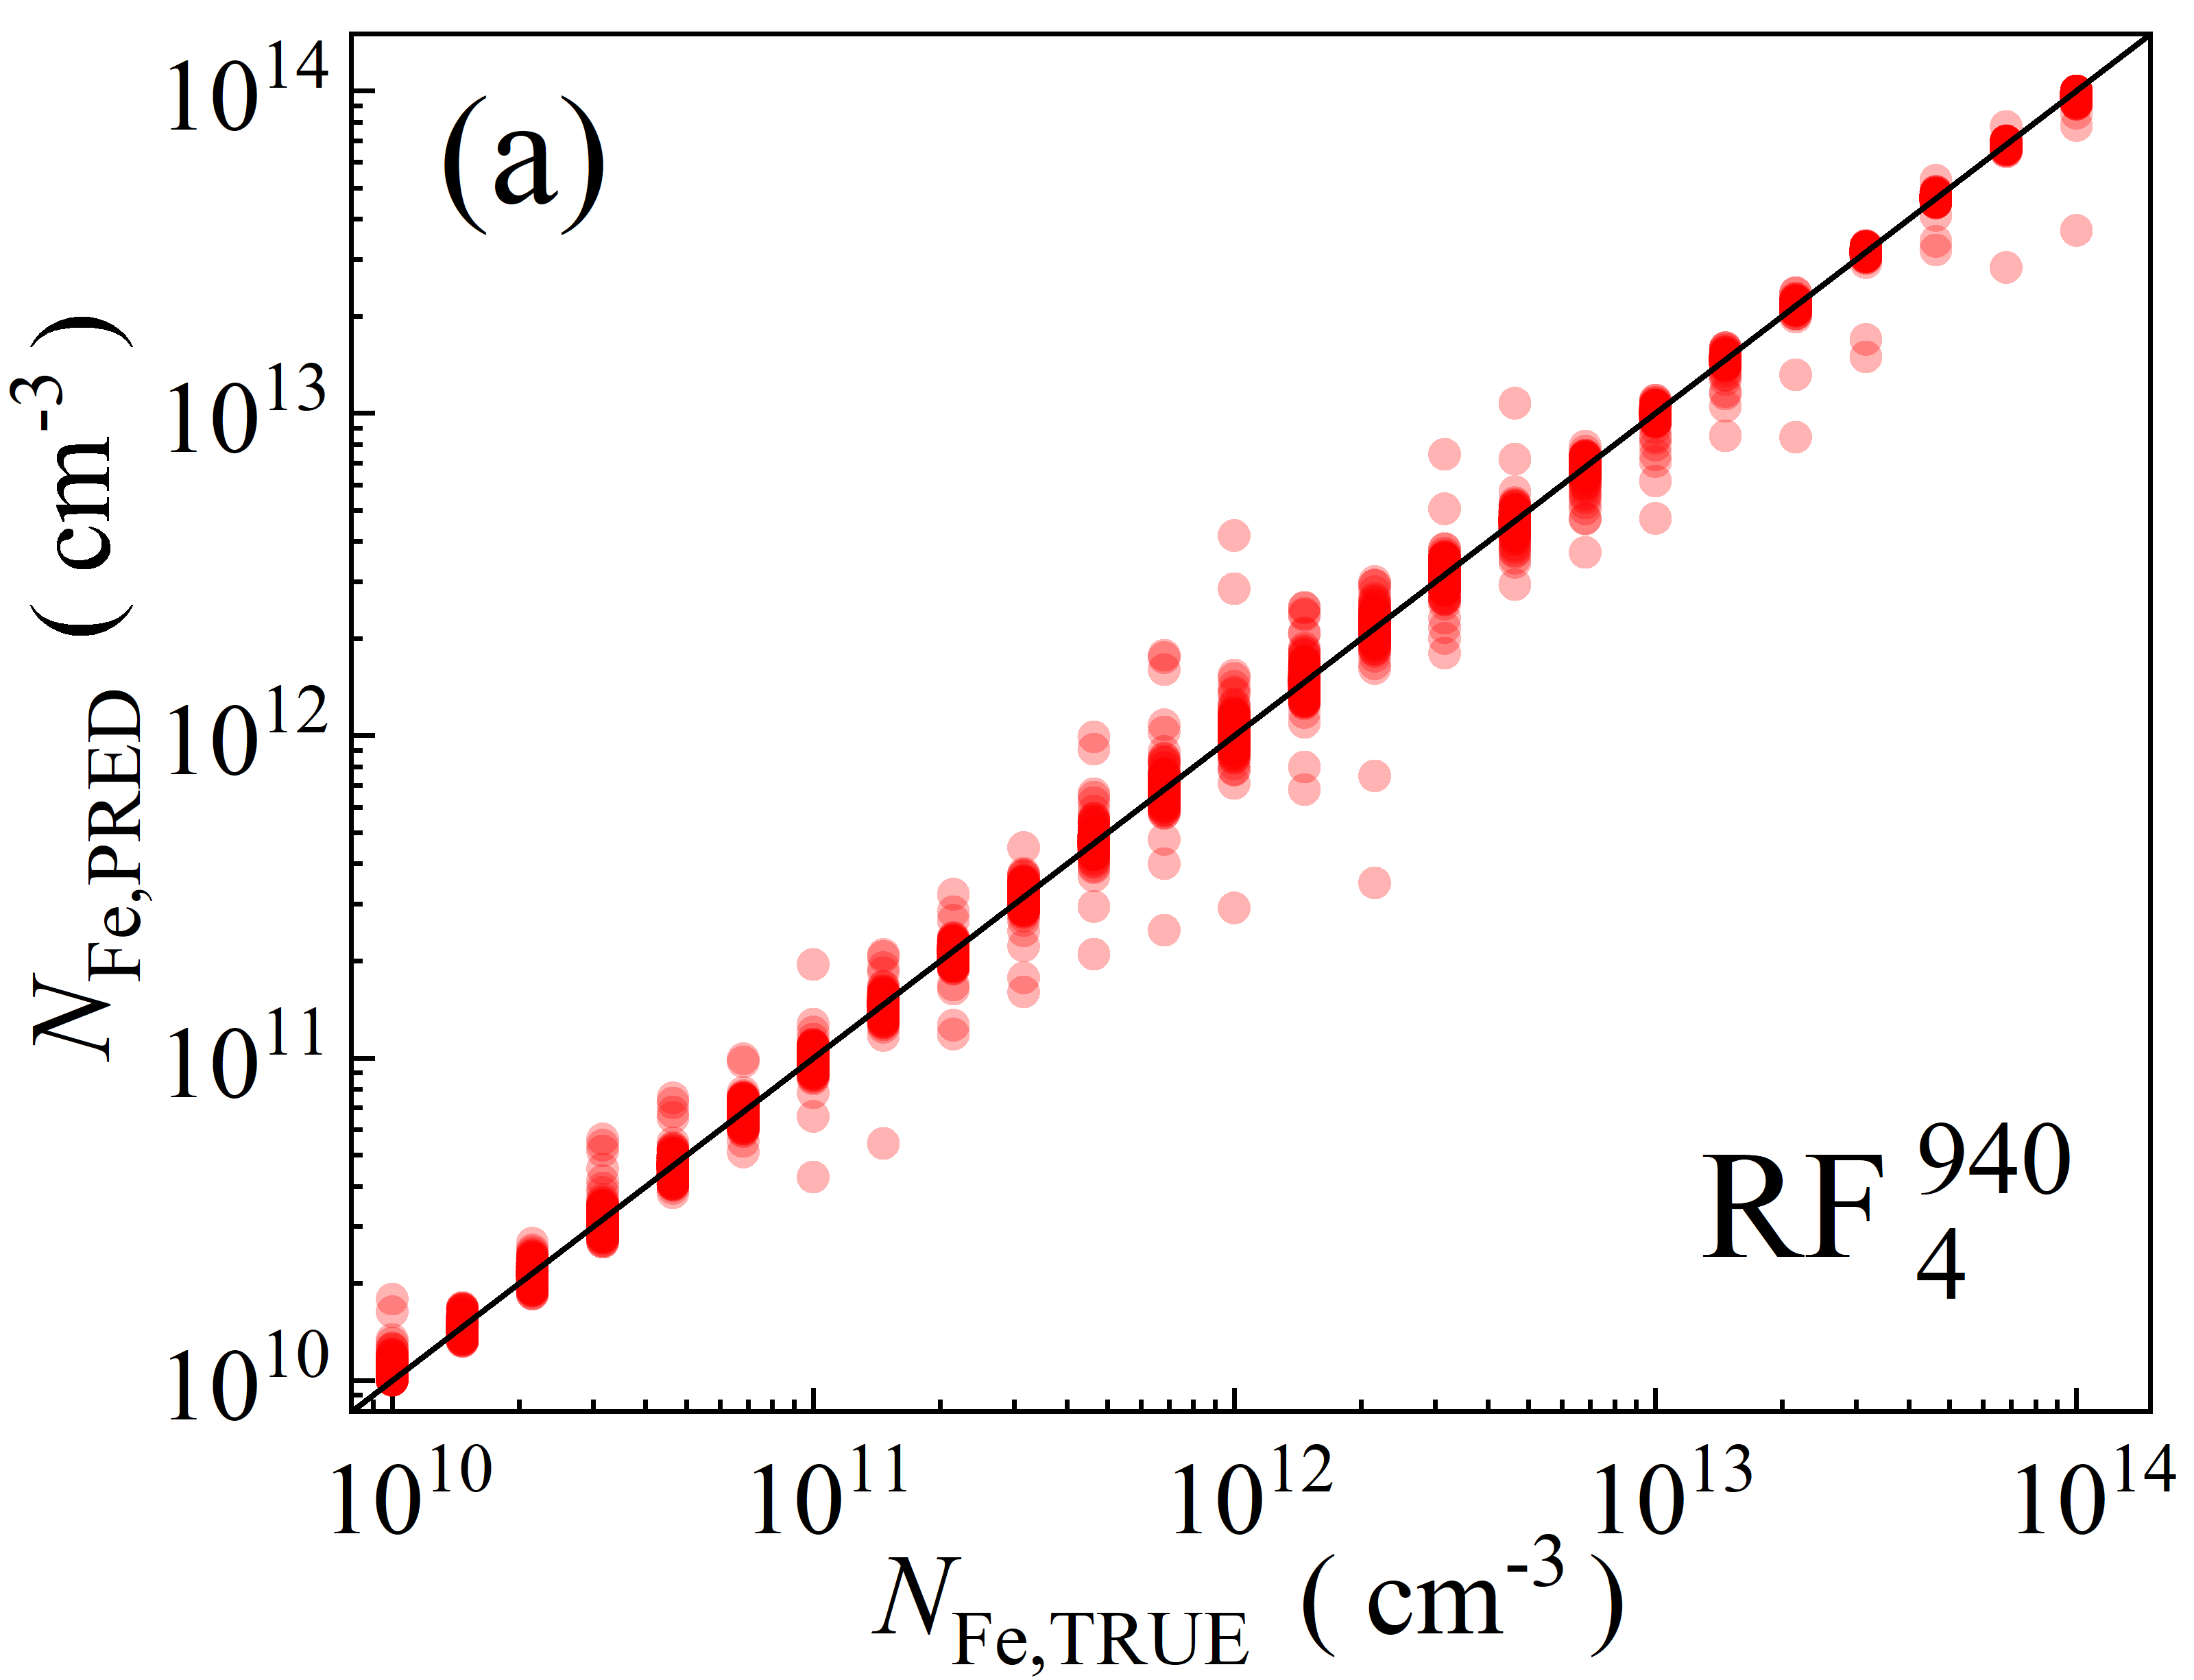
\includegraphics[width=0.4\linewidth]{Fig3a.png}
     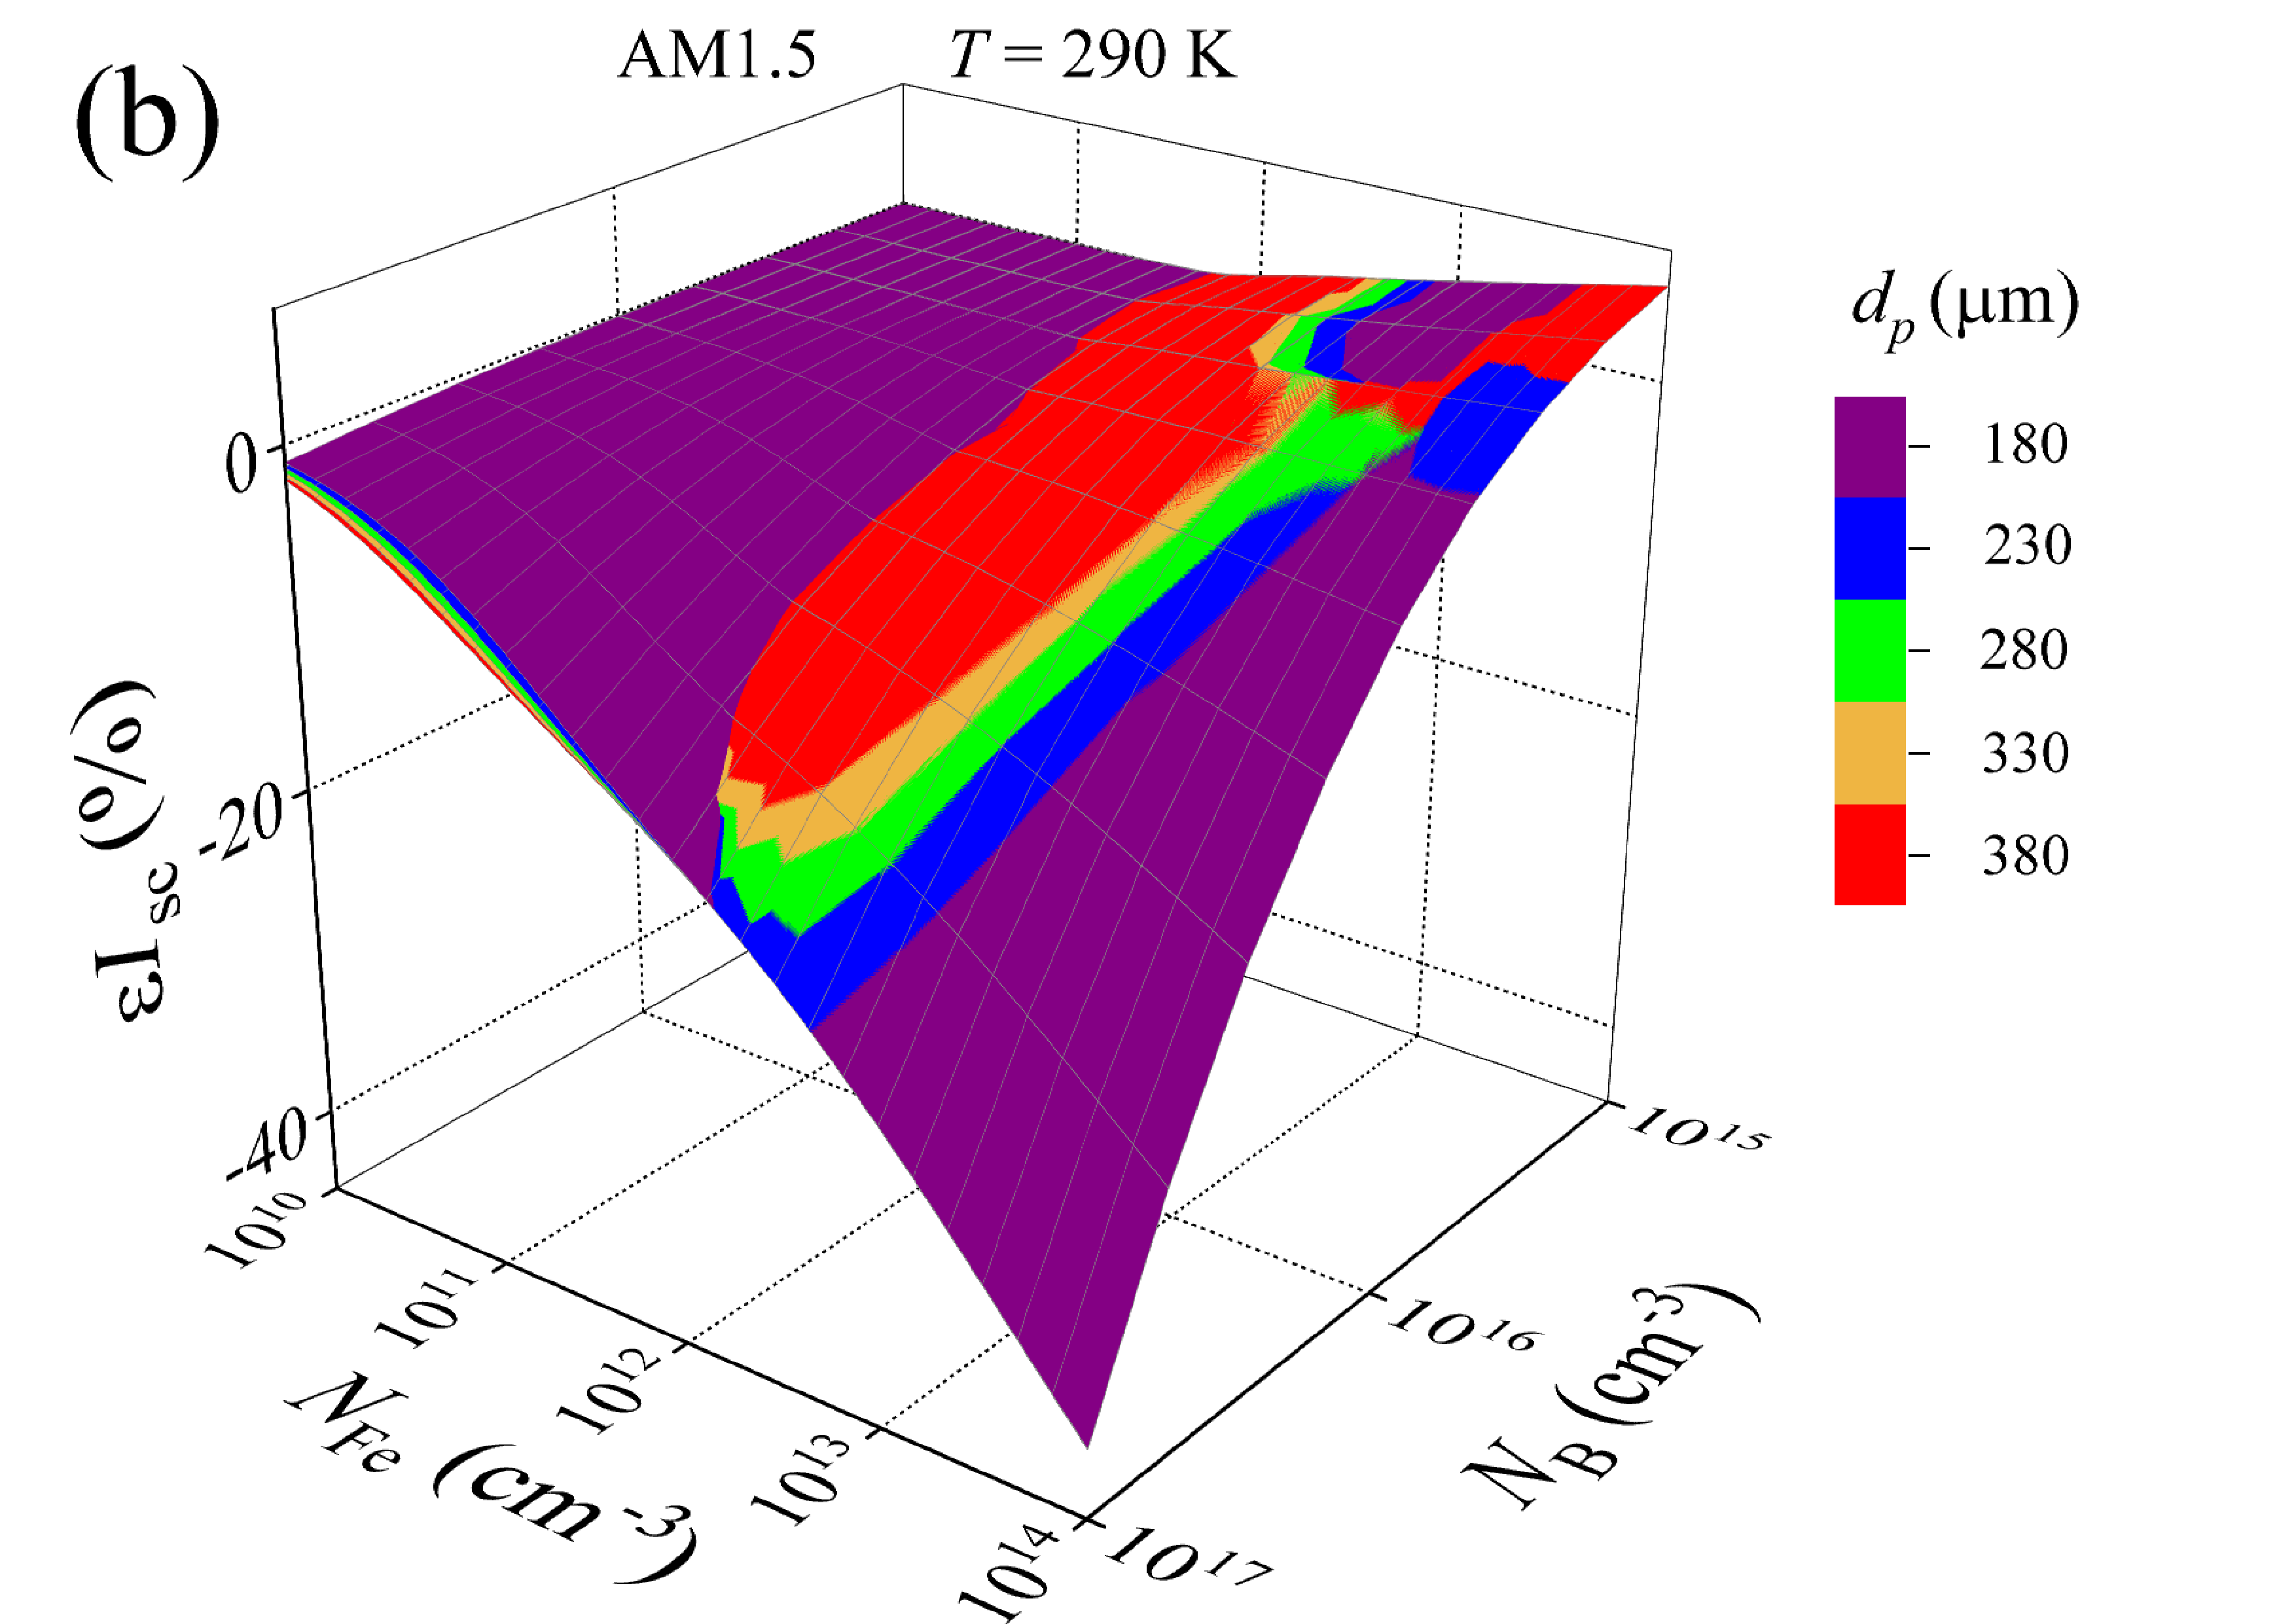
\includegraphics[width=0.4\linewidth]{Fig3b.png}
	  \caption{Dependencies of AI change in migration energy on US intensity
      for various frequencies.
       [Fe], $10^{13}$~cm$^{-3}$: 1.0 (a), 4.2 (b).
       AW type: longitudinal (a), transverse (b).
       $T=340$~K.
       The marks are experimental results,
       the lines are the linear fitted curves.
}\label{fig3}
\end{figure}

Fig.~\ref{fig4}a summarizes the $\beta$ values obtained for different samples and frequencies.
One can see that the relationships between $\beta$ and $f_\mathrm{US}$ are approximately linear.
In the case of longitudinal waves, the frequency coefficient has a negative value,
with a modulus that exceeds the corresponding value obtained for transverse waves.
In the low-frequency range (several MHz),
longitudinal waves exhibit higher effectiveness,
whereas at high frequencies (>15~MHz),  transverse waves are more effective
in enhancing the association of pairs.
Notably, in the vicinity of 10~MHz, the changes in $\Delta E_\mathrm{US}$ are independent of the vibration type.


\begin{figure}
	\centering
     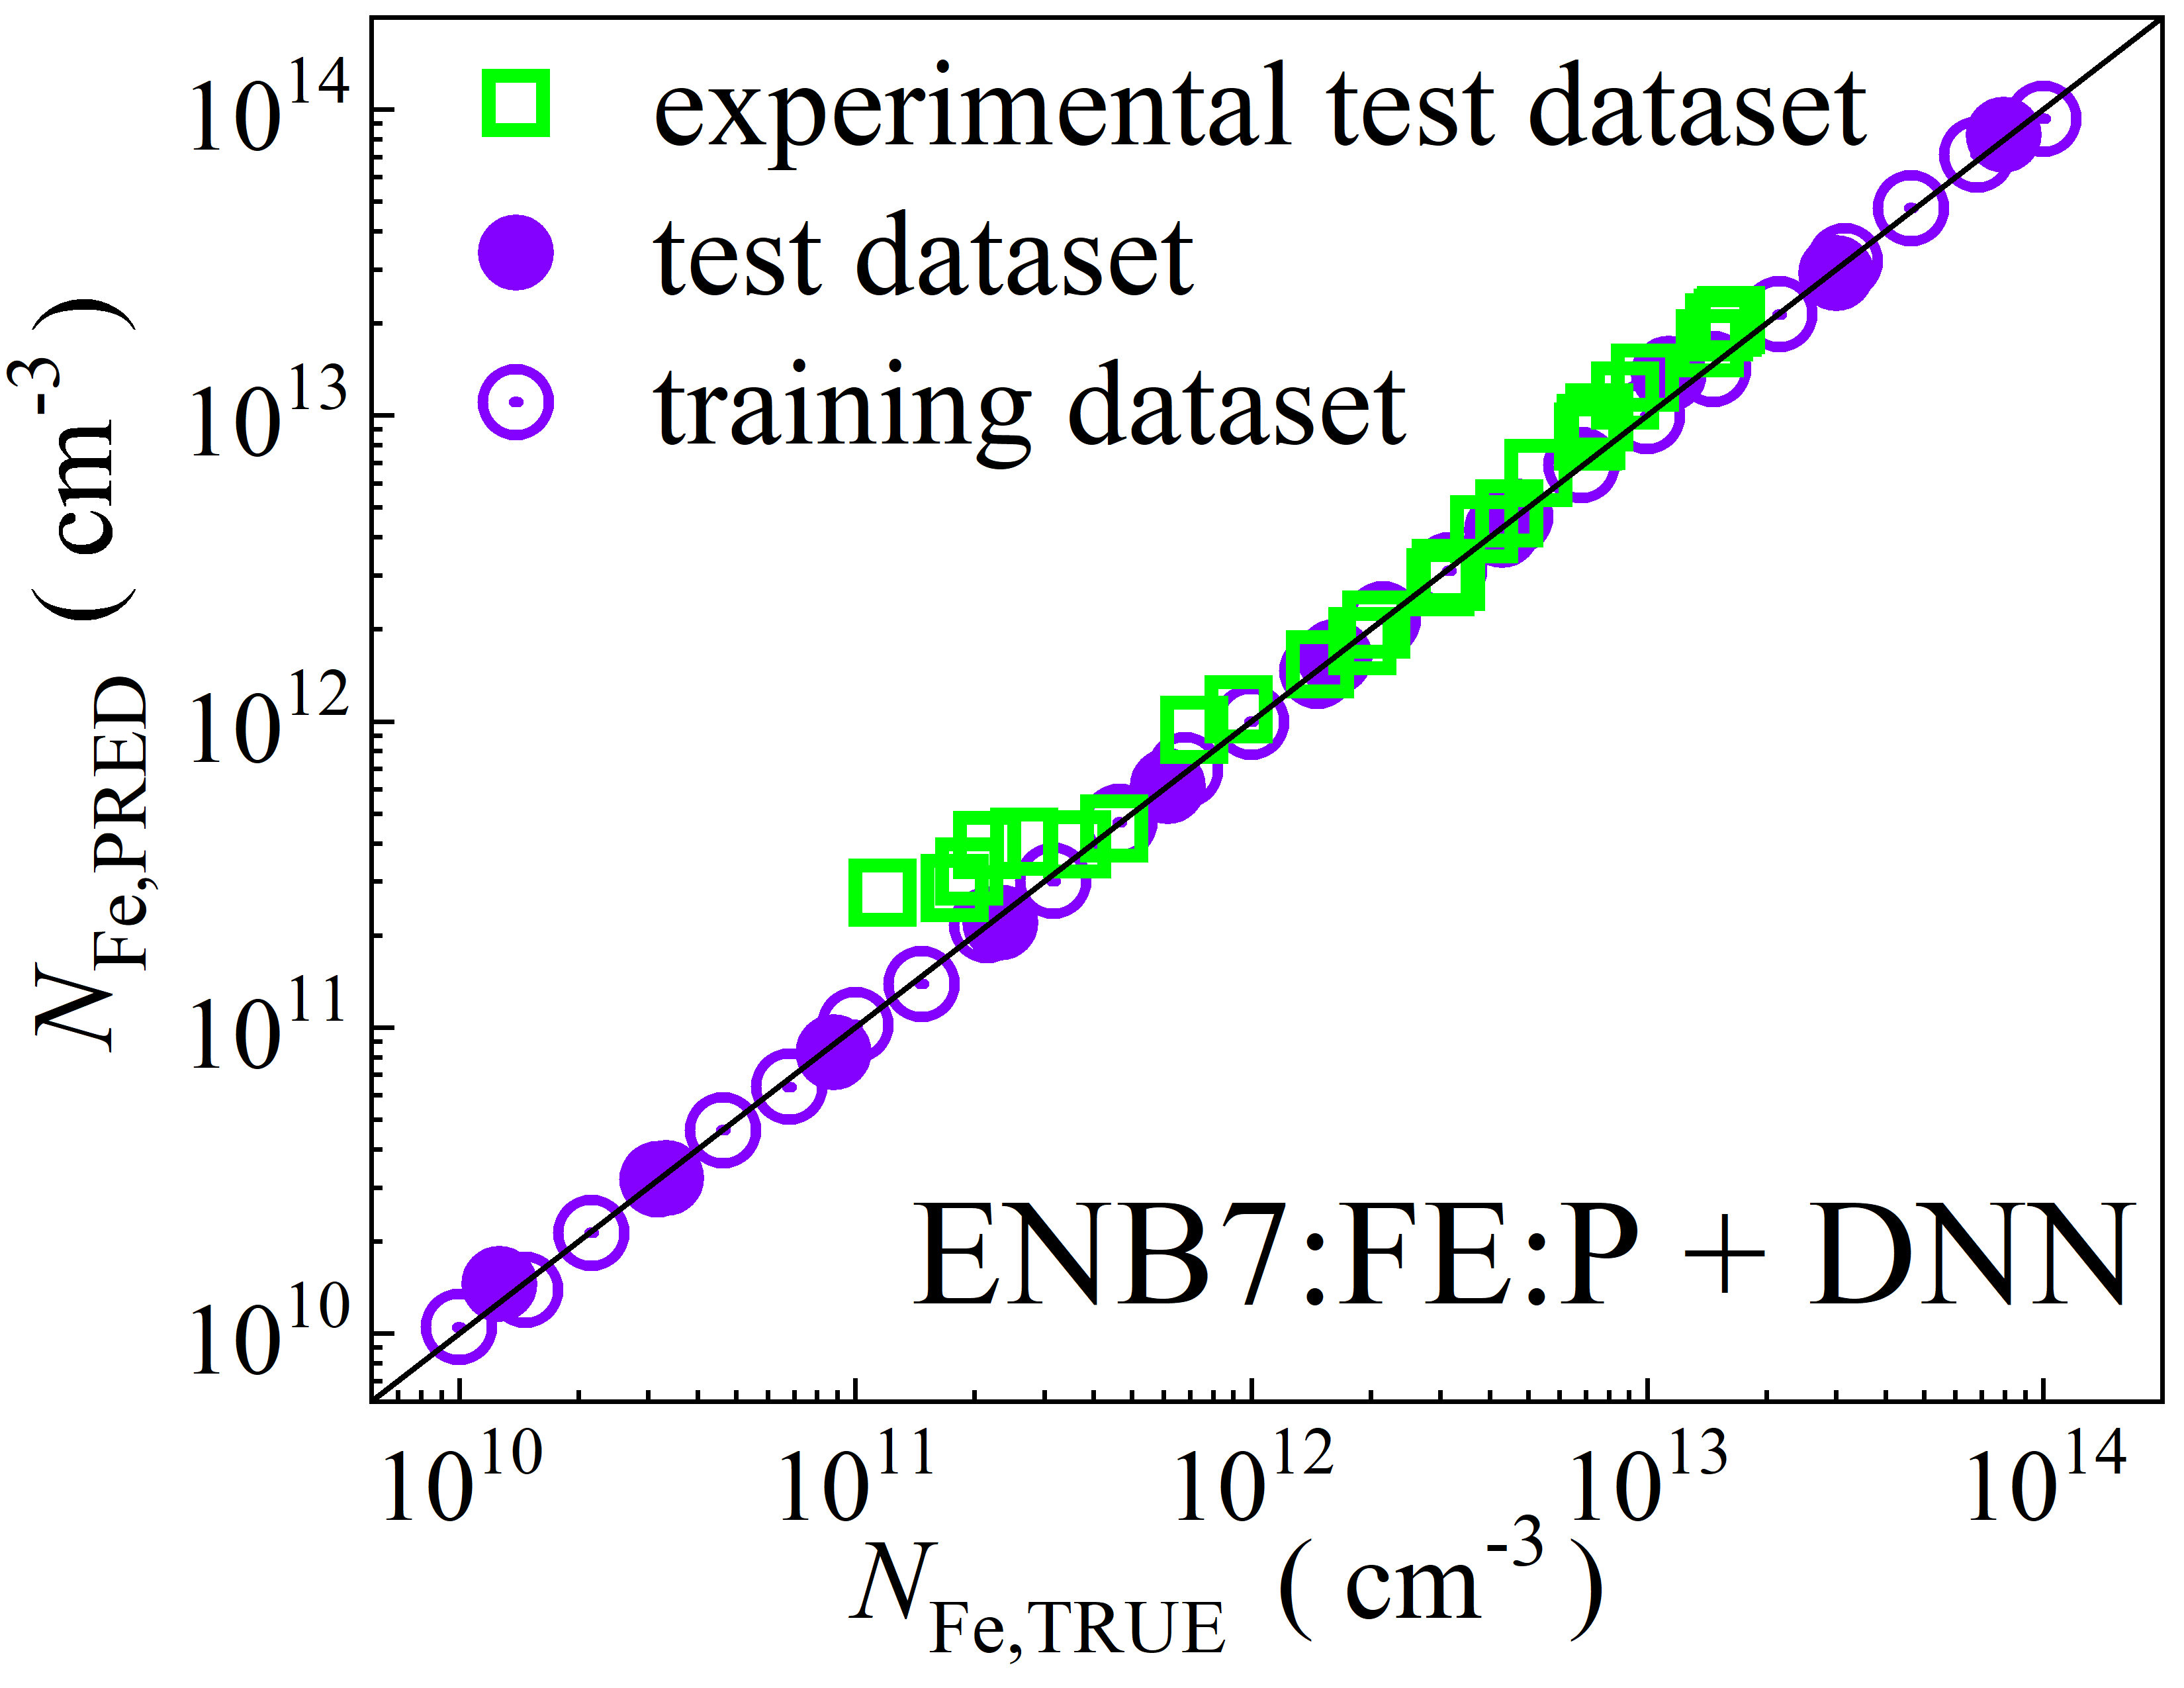
\includegraphics[width=0.4\linewidth]{Fig4a.png}
     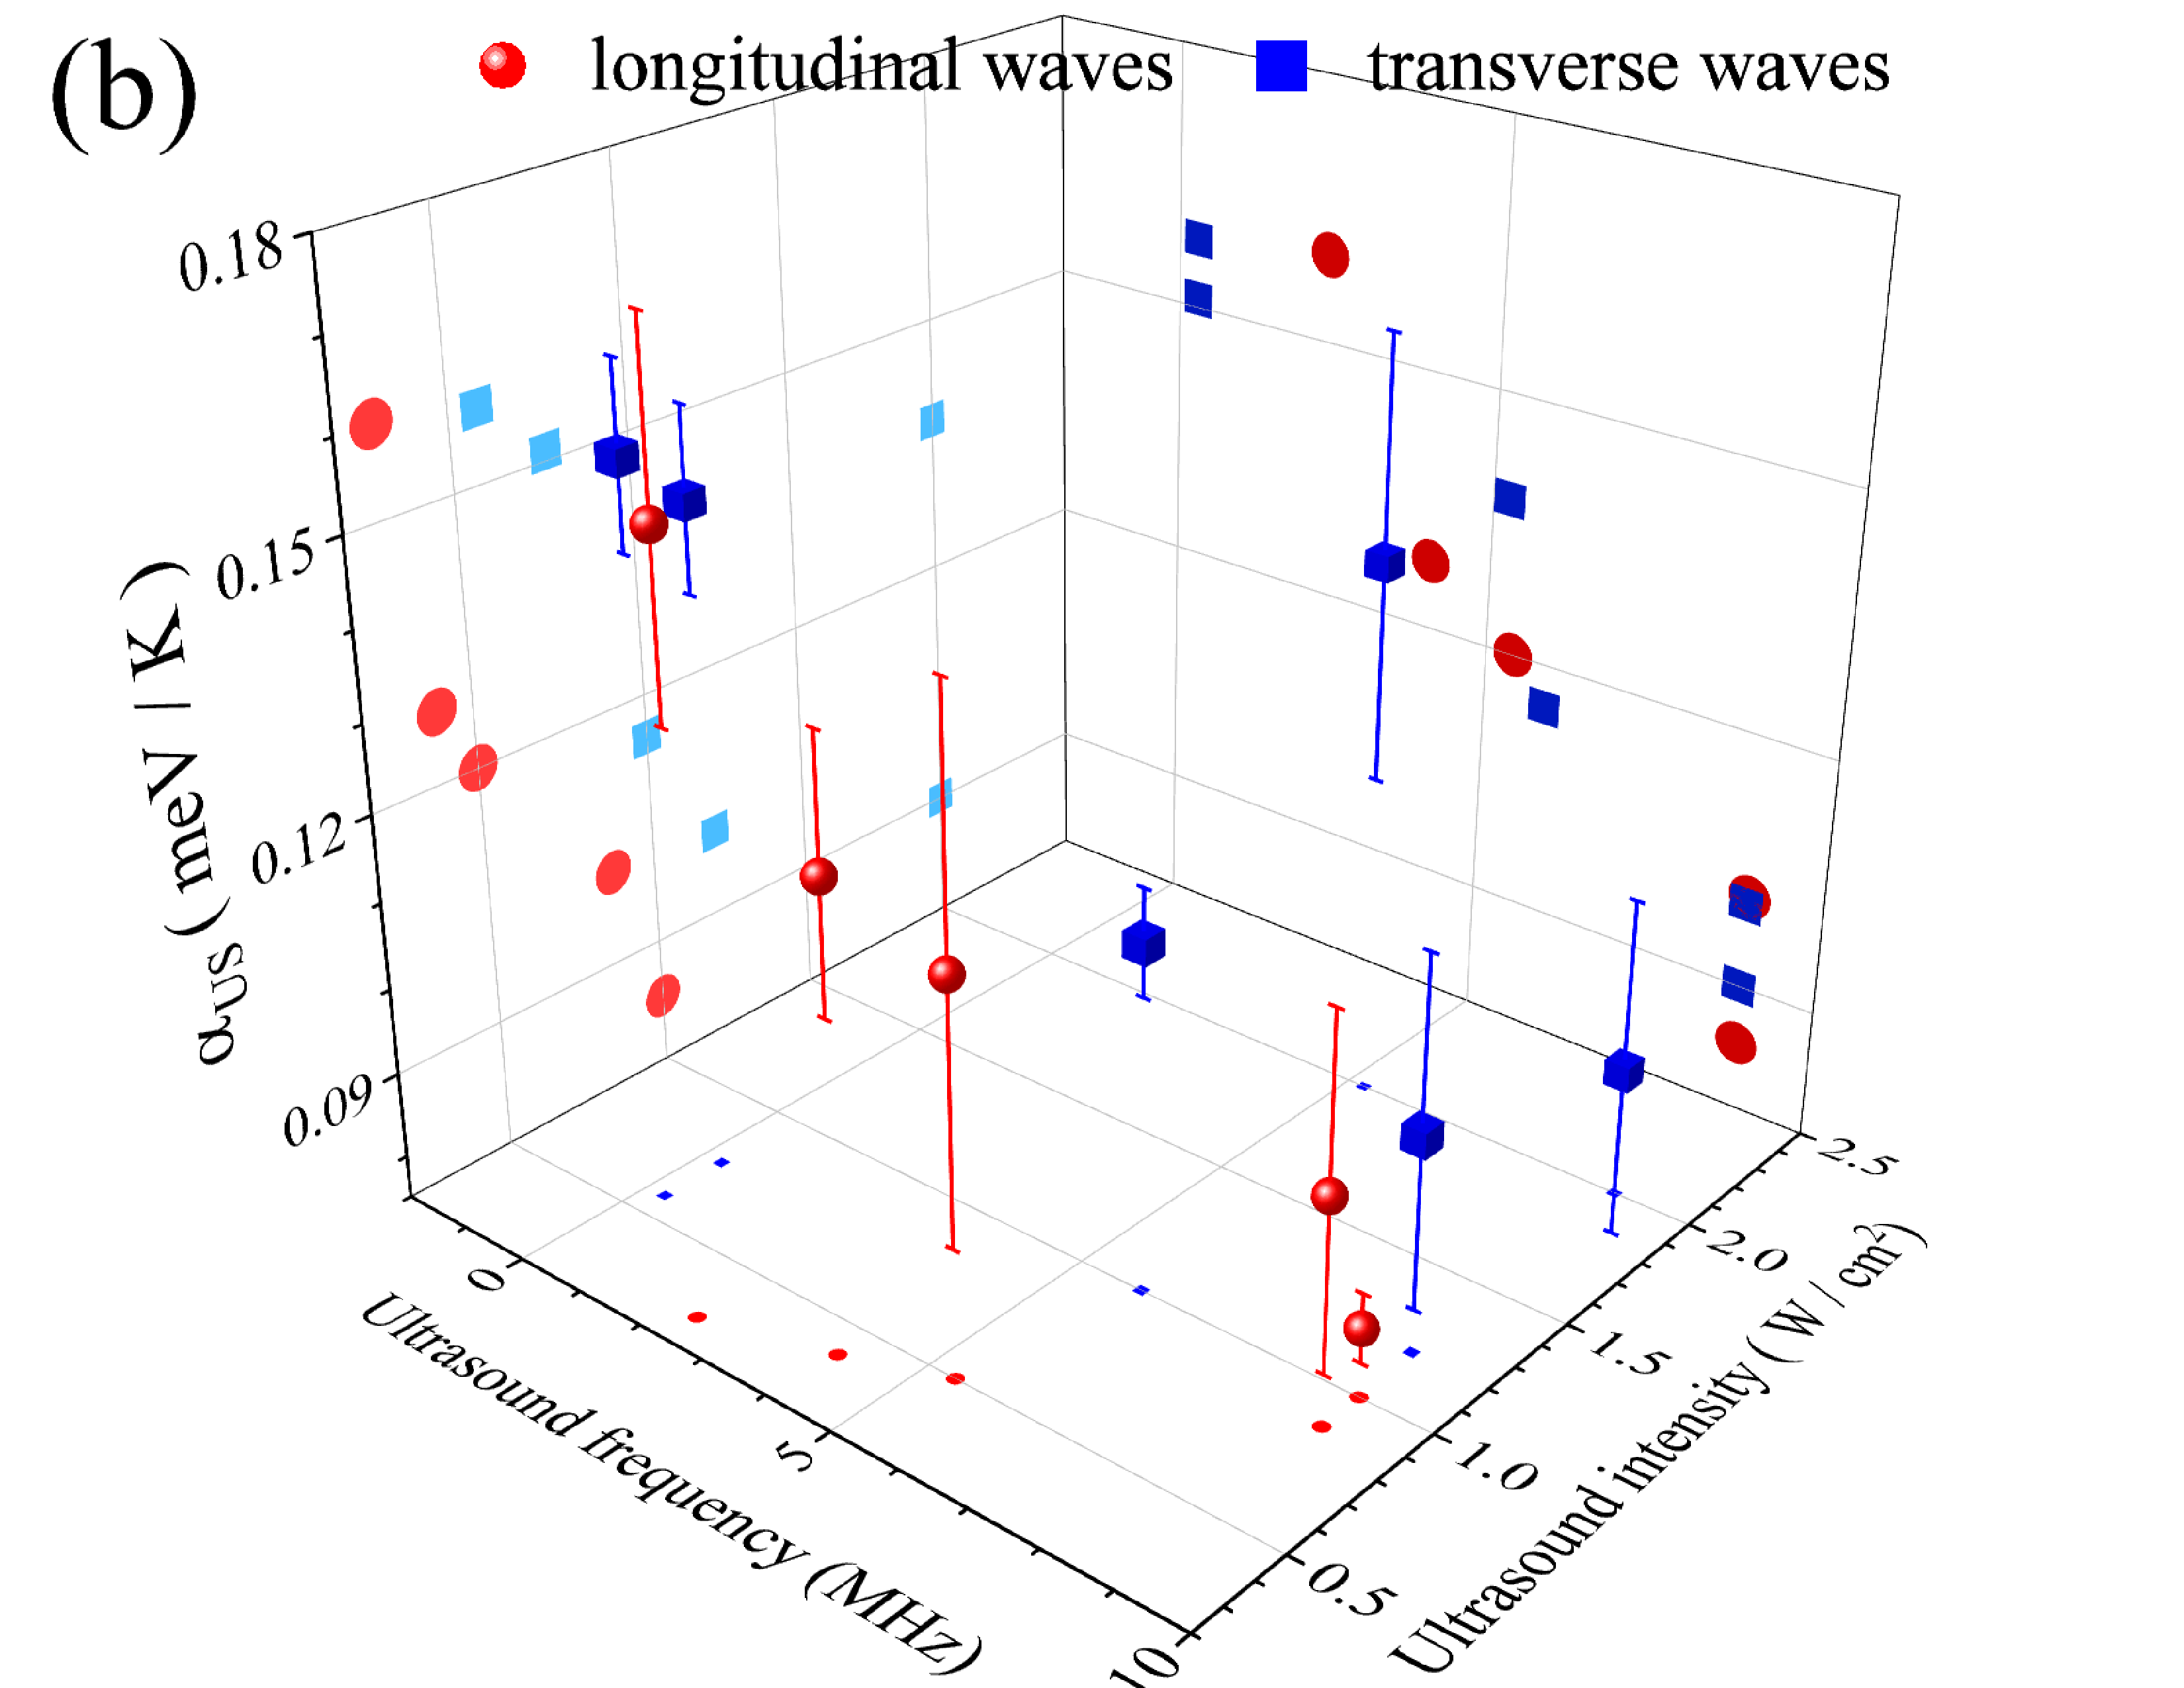
\includegraphics[width=0.4\linewidth]{Fig4b.png}
	  \caption{Dependencies of intensity coefficient (a)
       and temperature coefficient (b) of AI changes on US frequency and intensity.
       $\beta_\mathrm{US}$ values were obtained at $T=340$~K.
       AW type: longitudinal (red circles), transverse (blue squares).
       The numbers near the marks correspond to samples with different iron concentrations.
        [Fe], $10^{13}$~cm$^{-3}$: 0.20 (1), 0.37 (2), 0.7 (3), 1.0 (4), 1.9 (5), 
        3.0 (6), 4.0 (7), 4.2 (8), 4.3 (9).
}\label{fig4}
\end{figure}

As the temperature decreases, the AI effect diminishes --- see Fig.~\ref{fig5}.
The figure demonstrates that the temperature dependencies of $\Delta E_\mathrm{US}$ are similar for both wave types and are close to linear.
\begin{equation}
\label{eqEmT}
\Delta E_\mathrm{US}(T)@ W_\mathrm{US}=\Delta E_\mathrm{US}(0)+\alpha_\mathrm{US}T\,,
\end{equation}
where temperature coefficient $\alpha_\mathrm{US}$ depends on US frequency and intensity --- see Fig.~\ref{fig4}b.
The temperature coefficient exhibits the same dependence on frequency
for both transverse and longitudinal waves, with $\alpha_\mathrm{US}$ decreasing as the $f_\mathrm{US}$ increases.
The relationship between $\alpha_\mathrm{US}$ and $W_\mathrm{US}$ exhibits
similar behavior, both in terms of slope and independence from the wave type, as observed for $\alpha_\mathrm{US}(f_\mathrm{US})$.

\begin{figure}
	\centering
     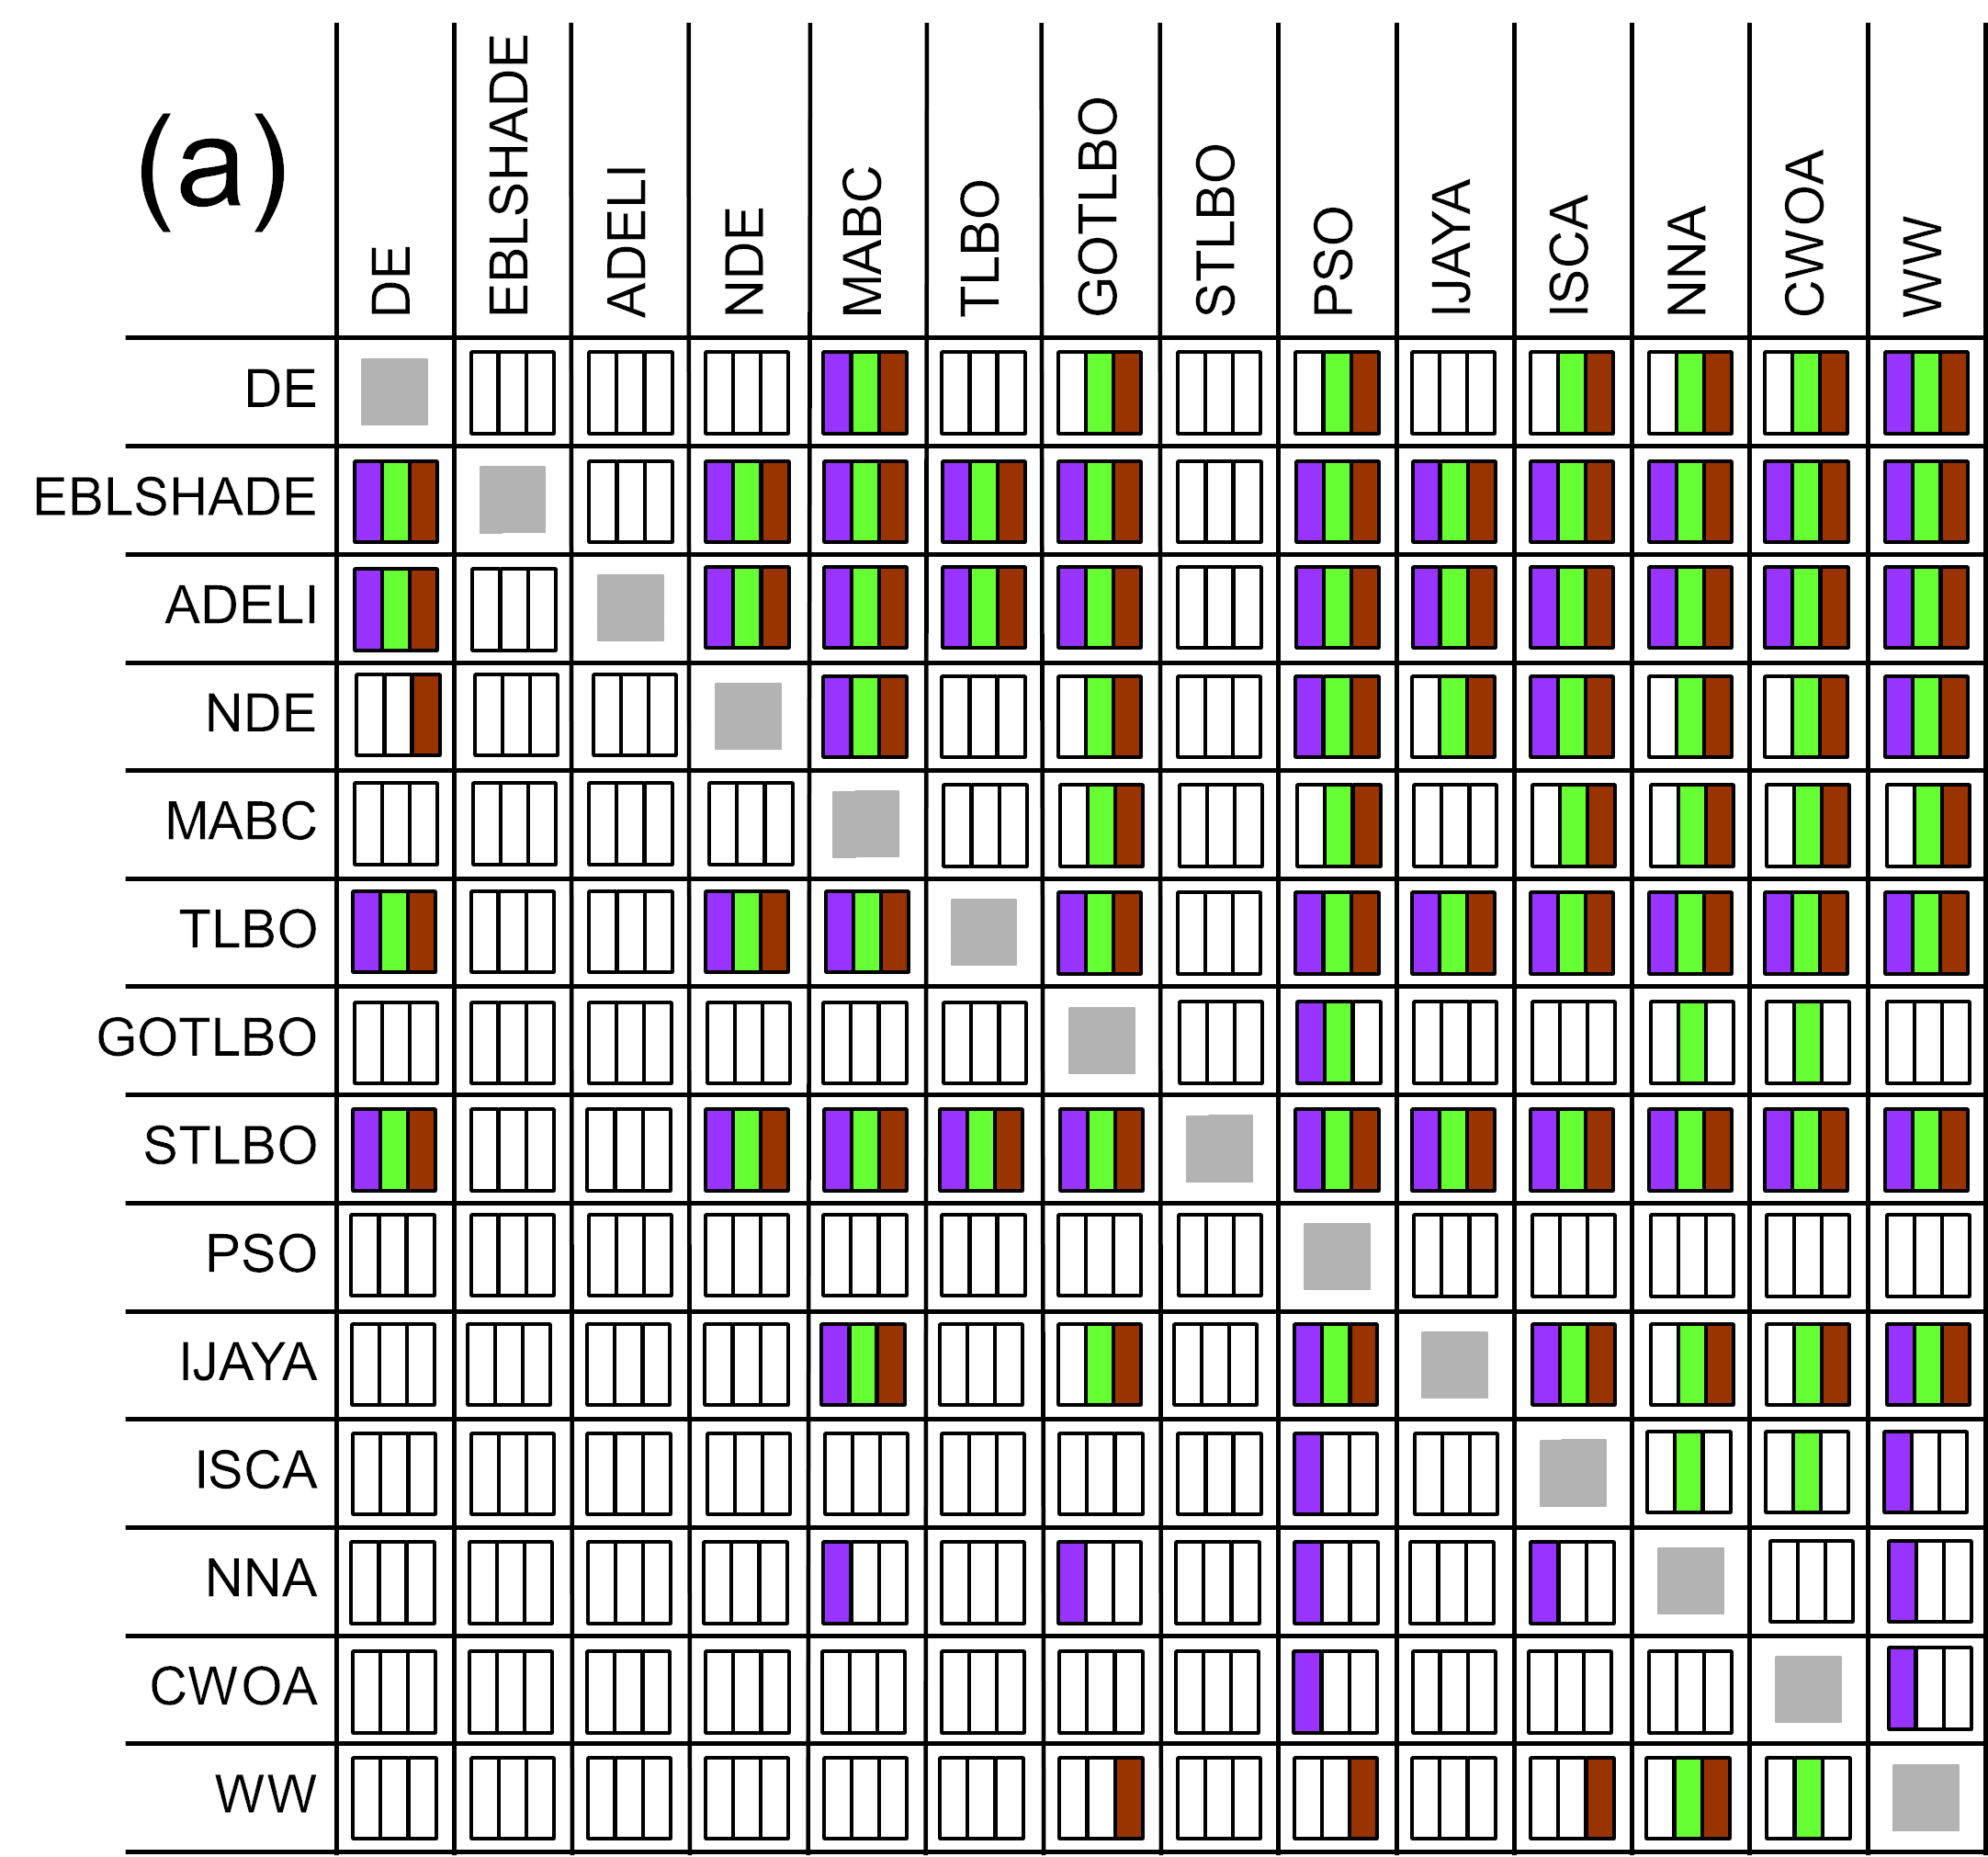
\includegraphics[width=0.4\linewidth]{Fig5a.png}
     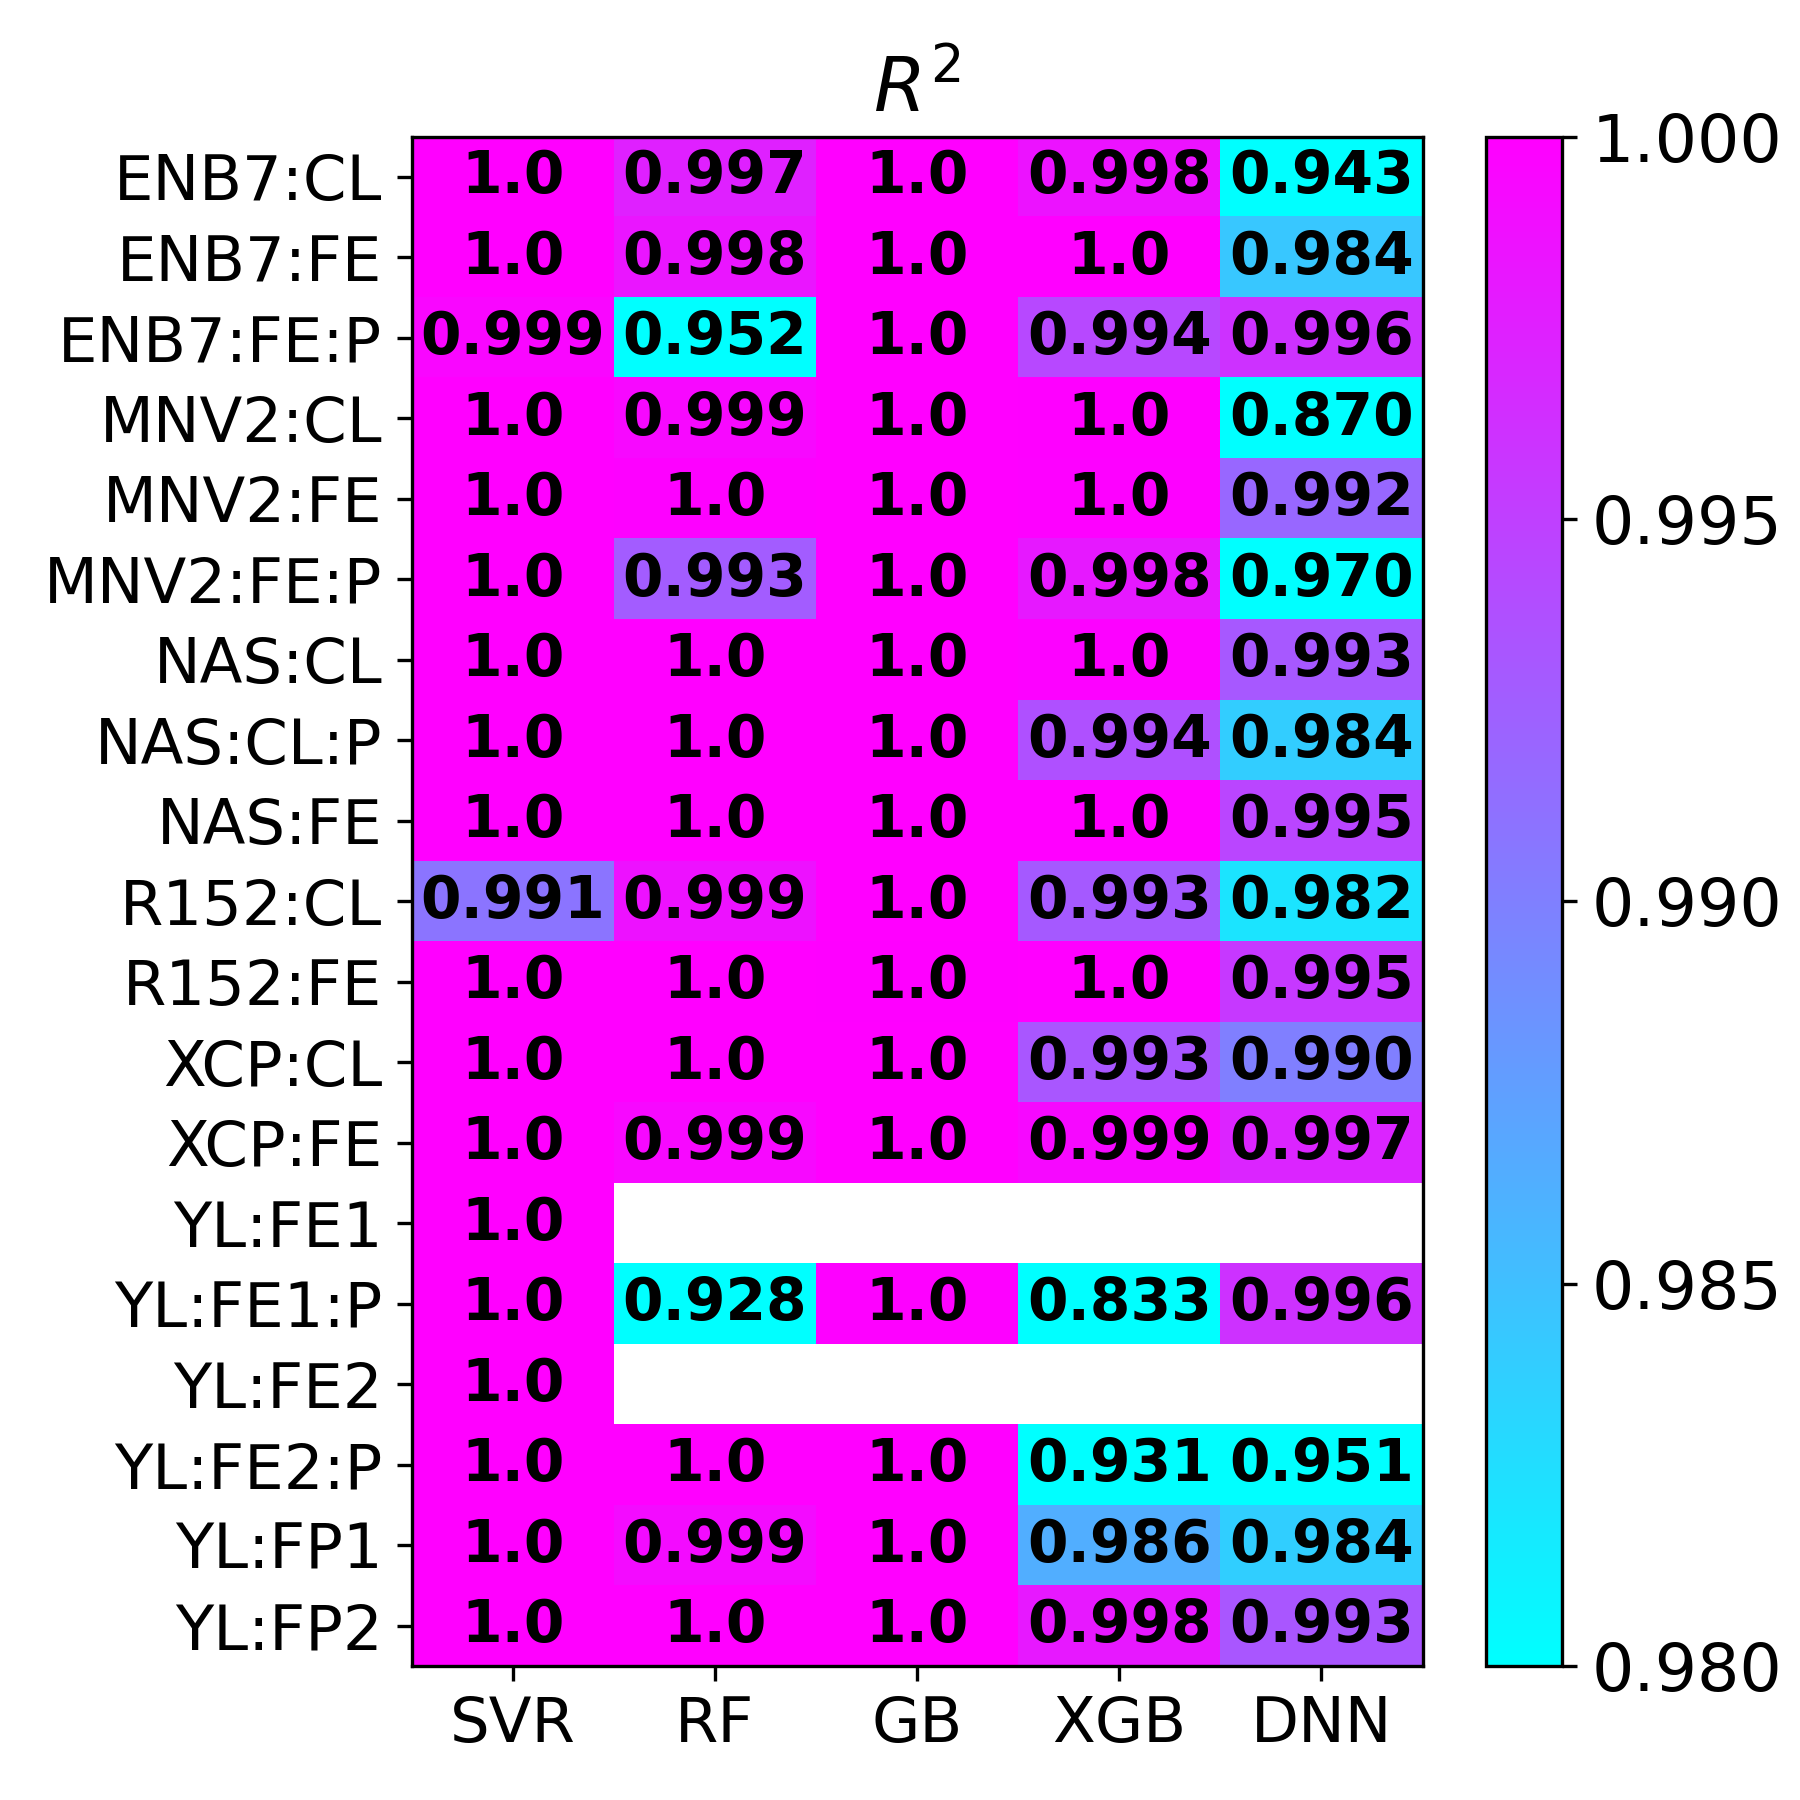
\includegraphics[width=0.4\linewidth]{Fig5b.png}
	  \caption{Temperature dependencies of $\Delta E_\mathrm{US}$.
       AW type: longitudinal (a), transverse (b).
       $f_\mathrm{US}$, MHz:  8.98 (1, 2), 5.04 (3),
       4.09 (4), 2.39 (5), 8.96 (6, 7), 5.94 (8), 5.23 (9), 0.31 (10, 11).
       $W_\mathrm{US}$, W/cm$^2$: 1.0 (1, 8), 0.87 (2), 0.1 (3), 0.4 (4), 0.3 (5), 2.0 (6, 9), 1.2 (7),
        0.76 (10), 0.58 (11).
        [Fe], $10^{13}$~cm$^{-3}$: 3.0 (1, 2, 4), 0.7 (3), 1.9 (5, 10, 11), 4.0 (6, 7, 9), 4.3 (8).
        The marks are the experimental results, the lines are the linear fitted curves.
}\label{fig5}
\end{figure}

Our findings indicate a complex interplay between the FeB pair association rate
and the acoustic field parameters.
Specifically, the effectiveness of reducing the iron ion migration energy
depends on temperature and ultrasound intensity,
while the corresponding coefficients exhibit frequency-dependent behavior.
The temperature coefficient exhibits similar dependencies for both transverse and longitudinal waves,
whereas the intensity coefficient exhibits opposing dependencies.

The most likely cause \cite{Olikh2021JAP} of the AI increase in the FeB association rate
is the transfer of energy from the thermal phonon ensemble,
which is out of equilibrium due to acoustic wave (AW) propagation, to diffused ions.
This mechanism has been discussed in Refs.~\cite{Pavlovich, Krevchik}.
On the one hand, according to Krevchik et al. \cite{Krevchik},
the diffusion activation energy $\Delta E_\mathrm{US}$ decreases proportionally
to $W_\mathrm{US}$, $T$ and should increase as the $f_\mathrm{US}$ value rises.
This expected behavior of $\Delta E_\mathrm{US}$  correlates with experimental results obtained for transverse waves.
On the other hand, impurity ion diffusivity should decrease due to an increase in
``polaron'' activation energy, as reported by Pavlovich \cite{Pavlovich}.
This effect may be the underlying cause of the negative value of $\beta_\mathrm{US}$ observed for longitudinal waves.
An alternative explanation may stem from the necessity of considering the direct oscillations of the impurity within the acoustic wave field.
In this scenario, the effect will be modulated by the deformation field that encloses the FeB pair
and results from the entire ensemble of atoms in Cz-Si.


\section{Positron Annihilation on FeB Complex: the Searching Estimations}

The difference in both the size of atoms and their electron structure in FeB complex
is the source of forming the strains and deformations in the crystal lattice of silicon.
The thermalized positron has the excursion length \cite{Krause1999} equal,
approximately, to 1000~{\AA} over the temperature range $\sim25$ to $300$~K
and thus may form a many-body electron-positron localized state at the
FeB complex in case its concentration is not very much lower than about $10^{15} – 10^{14}$~cm$^{−3}$.
The rate of this localization ($k$) with the consequent emission of annihilation
gamma-quanta out of the volume of FeB complex is determined by measuring the positron annihilation characteristics.
The latter are known to be determined by both the open volume and chemical nature of atoms involved in a defect \cite{Krause1999}.
The positron probing of defects becomes indispensable when other methods
(e. g., such as EPR and IR spectroscopy), are not informative ones.
In addition, also one may point out to the NMR and acoustic nuclear magnetic resonance
that are not used for studying nuclei having zero nuclear spin.


\noindent \textbf{Positron Trapping.}
To detect acoustic loading on a defect by positron annihilation
one needs to have positron states related to it.
A propensity of the thermalized positron to be localized in the region of negative effective charge
related to the impurity atoms of different nature together
with the open volume of a defect is generally accepted to describe by the trapping model \cite{Brandt1974}:
\begin{equation}\label{eqA1}
  k=\lambda_0\frac{\eta}{1-\eta}\cong\lambda_0\frac{\tau_\mathrm{av}-\tau_0}{\tau_\mathrm{max}-\tau_\mathrm{av}}\,,
\end{equation}
where the resulting probability of  2–gamma annihilation
is measured assuming that the positron trapping rate $k$ allows one
to determine conditional probability $\eta$ of the event
of 2–gamma annihilation of $e^+e^-$ pair in the centers studied \cite{Brandt1974,Arutyunov2013}:
\begin{equation}\label{eqA2}
  \eta=\frac{k}{\lambda_0+k}\,.
\end{equation}
The averaged positron lifetime $\tau_\mathrm{av}$ is expected
to depend on the acoustic loading, and $\tau_0$ is a positron lifetime out of a defect;
this value is not measured.
As $\tau_0$ magnitude it is generally accepted to use so-called $\tau_\mathrm{bulk}$ value which is, e.g.,
determined experimentally for a defect--``free'' material.
The cross-section of positron localization with the subsequent 2--gamma annihilation $\sigma_+$ determines the $k$ value:
\begin{equation}\label{eqA3}
  \sigma_+=k/C\,,
\end{equation}
where $C$ is the coefficient of localization of positron pair at the center \cite{Krause1999};
$C=[\mathrm{FeB}]\times v_+$
($v_+$ is the velocity of positron on its excursion length $\sim (4\tau D_+)^{0.5}$
where $\tau$ and $D_+$ are the positron lifetime and the positron diffusion coefficient, respectively \cite{Krause1999,Brandt1974}.
Over the range of concentrations [FeB] from $2\times10^{13}$~cm$^{−3}$ to $\sim10^{14}$~cm$^{−3}$
the $k$ value $k\{[FeB]; \sigma_+ = 10^{−12} \mathrm{cm}^2\}$
increases from $\sim0.5$ to $\sim1$~ns$^{−1}$.
In the case of increase of the positron trapping cross section up to $10^{−11}$~cm$^2$
for the same range of concentrations of defects the value of the positron trapping rate increases from $\sim2$ to $\sim10$~ns$^{−1}$.
This range of the $k$ magnitudes is well detected using both PALS and CDB.

The $k$ value may turn out to be more pronounced due to yet much larger values of cross-sections.
It should be noted in this connection that large cross sections $\sim\!3.32\times10^{–11}$~cm$^2$
and $\sim\!10^{–10}$~cm$^2$  related to excitonic Auger capture of holes and multiphonon emission capture,
respectively, have been reported for the FeB complex \cite{Paudyal2009,Istratov1999}.

Thus, one can expect observing the emission of annihilation radiation modulated by USL on FeB centers
whose association was shown to be accelerated in the solar cells \cite{Olikh2022:JMatSci}.
Special interest in this connection is a paradoxical divergence in the frequency dependency of reduced
energy barrier for Fe ion migration $E_m \xrightarrow{\mathrm{US}} E_{m,0}-\Delta E_\mathrm{US}$
when using longitudinal and transverse waves.
This intriguing dependency observed suggests forming the anisotropic deformation field ambient FeB complex
which consists of the atoms of Si, Fe, B and others, such as oxygen and carbon in Cz-grown silicon.


\noindent \textbf{Elementally-Specific Annihilation Radiation.}
The ion cores of different chemical nature in the atomic environment of the positron
makes the emission of the high-momentum annihilation gamma-quanta to be elementally specific one inasmuch
as the wave functions of the ion core electrons retain to a great extent their atomic character in solids.
The data obtained for these electron-positron states by the angular correlation of annihilation radiation (ACAR)
of high resolution for the poly-crystalline metallic Fe (in its $\gamma$--phase),
as well as for so-called $\beta$--B and dislocation-free $n$–type FZ–Si [111] single crystal are shown in Fig.~\ref{fig6}.
The electron-positron ion radii $r_m$ obtained by these data are close to the values of ionic radii $r_i$:
for different coordination numbers $r_i(\mathrm{Fe}^{2+}; \mathrm{Fe}^{3+})$ and $r_i(\mathrm{Si}^{4+})$ values
range 0.63 to $0.92\times10^{−8}$~cm and $0.4$ to $0.54\times10^{−8}$~cm, respectively;
the ionic radius of boron $r_i(\mathrm{B}^{3+})$ is equal to $\simeq0.27\times10^{−8}$~cm \cite{Suchet1965,Rahm2016}.
The $r_m$(B) value is larger than the length of ionic radius $r_i(\mathrm{B}^{3+})$ as the maximum overlapping of the ion core
 electrons and positron wave functions \cite{Ferrell1956} is shifted outwards the ion core of B atom more effectively than it takes place for ion cores of Fe and Si atoms.


\thisfloatsetup{capposition=beside,%
      capbesideposition={right,center},
      capbesidewidth= 0.6\linewidth,
      floatwidth= 0.38\linewidth
  }

\begin{figure}
	\centering
%     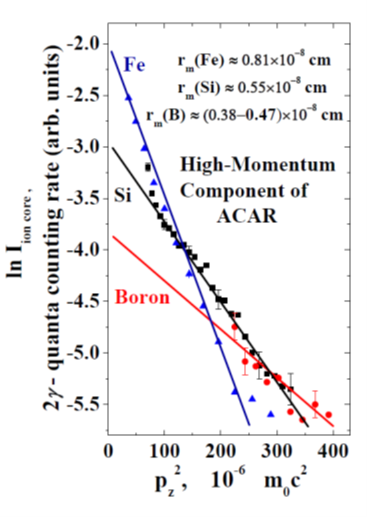
\includegraphics[width=0.35\linewidth]{Fig6.png}
     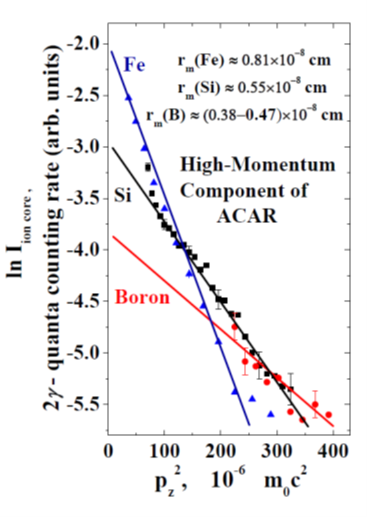
\includegraphics[width=\linewidth]{Fig6.png}
	  \caption{The high-momentum component of the elementally-specific ACAR spectra
        obtained by the spectrometer of high geometrical angular resolution $\Delta \approx 0.48 \times 10^{-3}\,m_0\,c$
        ($m_0$ and $c$ are the electron mass and the light velocity, respectively).
        The span between detectors of ACAR installation was 4.25~meters, and the collimating slits had 2~mm width.
        The measurements were performed at room temperature and their results are given
        for boron (dots), silicon (squares), and iron (triangles).
        The electron-positron ionic radus $r_m$ were restored (see \cite{Arutyunov2016,Arutyunov2006,Arutyunov2008} for more detail).
        The lines are the results of fitting, the slopes of the linear functions are obtained with the accuracy
        which is characterized by the standard deviation / the Pearson’s coefficient, respectively:
        0.042/0.998 (Fe), 0.114/0.956 (B) and 0.101/0.99 (Si).\\
        The many-body electron positron state at FeB complex modulated by USL must generate
        similar spectrum of high-momentum components of 2–gamma annihilation radiation.
}\label{fig6}
\end{figure}

The resulting emission of 2–gamma annihilation radiation out of Fe, Si, and B subvalent and ion core electron states
to be probed with positrons follows the squares under the lines in Fig.~\ref{fig6}.
%Similar trend should be observed for the many-body electron-positron state at FeB pair including its complexes with common impurities in Cz-Si.
Similar trend would create a pattern with different contributions of elementally specific ACAR
and should be observed for the many-body electron-positron state at FeB pair including its complexes with common impurities in Cz-Si.
The relative contributions of these elementally-specific channels of annihilation radiation depend on the both configuration and symmetry of FeB complex,
thus manifesting themselves in the mutually interrelated both the average positron lifetime,
$\tau_\mathrm{av}$, and conditional probabilities, $\eta$;
see Eq.~\ref{eqA1} and Eq.~\ref{eqA2}.
The numeral values of these parameters will be changed under USL,
thus allowing one to observe the acoustic-positron annihilation phenomena.
Instead of a high-precision ACAR measurements, the CDB may be used for detecting the electron-positron annihilation in the ion cores
of atoms involved in the microstructure of defects, with the subsequent analysis of $S$-$W$-parameters of CDB spectra \cite{Krause1999}.

\section{Conclusion}

The effects of longitudinal and transverse acoustic waves on FeB pairing in silicon have been investigated experimentally.
The results show that the efficiency of ultrasonic influence on the association process significantly depends on the type of wave.
The findings reveal a controlled variability in the effect of ultrasound on the generation and evolution of structural defects.
The characteristics of positron annihilation on the FeB complex have been analyzed,
and the feasibility of using positron annihilation spectroscopy under ultrasonic loading has been demonstrated.
Thus, ultrasound can be an effective tool for controlling defect characteristics in semiconductors.



\section{Acknowledgments}
N. A. is thankful to DAAD for partial support of this work.
O. O. is thankful to NRFU (Pr. No. 2023.03/0252) for partial financial support of this work.


\begin{thebibliography}{99}

\bibitem{Ostapenko1999} S. Ostapenko: Appl. Phys. A: Mater. Sci. Process. Vol. 69 (1999), p.~225

%\bibitem{Ostap:PhotoLum} J. Koshka, S. Ostapenko, T. Ruf and J. M. Zhang: Appl. Phys. Lett. Vol. 69 (1996), p.~2537

\bibitem{BORKOVSKA2003} L.V. Borkovska, M.P. Baran, N.O. Korsunska et al.: Phys. B Condens. Matter Vol. 340–342 (2003), p.~258

\bibitem{Bahar2003} A. El-Bahar, S. Stolyarova, A. Chack et al.: Phys. Status Solidi A Vol. 197 (2003), p. 340

\bibitem{RITTER2008} U. Ritter, P. Scharff, V.V. Kozachenko et al.: Chem. Phys. Lett. Vol. 467 (2008), p. 77

\bibitem{Wosinski} T. Wosinski, A. Makosa and Z. Witczak: Semicond. Sci. Technol. Vol. 9 (1994), p. 2047

\bibitem{UST:OstrovCsI} I. Ostrovskii, N. Ostrovskaya, O. Korotchenkov and J. Reidy: IEEE Trans. Nucl. Sci. Vol. 52 (2005), p. 3068

\bibitem{UST:LED_SM} O. Konoreva, Ya. Olikh, M. Pinkovska et al.: Superlattices Microstruct. Vol. 102 (2017), p. 88

\bibitem{GORB2020} A.M. Gorb, O.A. Korotchenkov, O.Ya. Olikh et al.: Solid-State Electron. Vol. 165 (2020), 107712

\bibitem{Gorb2010} A.M. Gorb, O.A. Korotchenkov, O.Ya Olikh and A.O. Podolian: IEEE Trans. Nucl. Sci. Vol. 57 (2010), p. 1632

\bibitem{Litovchenko2015} V. Litovchenko, V. Melnik and B. Romanjuk: Ukrainian Journal of Physics Vol. 60 (2015), p. 64

\bibitem{ROMANJUK2005MatSci} B. Romanjuk, V. Kladko, V. Melnik et al.: Mater. Sci. Semicond. Process. Vol. 8 (2005), p. 171

\bibitem{Wang:JLum} W. Wang, F. Huang, Y. Xia and A. Wang: J. Lumin. Vol. 128 (2008), p. 199

\bibitem{US:ZnOfilm} S. Fujita, K. Kaneko, T. Ikenoue et al.: Phys. Status Solidi C. Vol. 11 (2014), p. 1225

\bibitem{YOlikhTPL2011} Ya.M. Olikh  and  M.D. Tymochko: Tech. Phys. Lett. Vol. 37 (2011), p. 37

\bibitem{Ostrovskii2001} I. Ostrovskii, O. Korotchenkov, O. Olikh et al.: J. Opt. A: Pure Appl. Opt. Vol. 3 (2001), p. S82

\bibitem{buyanova1994} I.A. Buyanova, S.S. Ostapenko, A.U. Savchuk and M.K. Sheinkman: Mater. Sci. Forum Vol. 143 (1993), p. 1063

\bibitem{belyaev1994} A.E. Belyaev, H.J. von Bardeleben, M.L. Fille et al.: Mater. Sci. Forum Vol. 143 (1993), p. 1057

\bibitem{Korotchenkov1995} O.A. Korotchenkov and H.G. Grimmliss: Phys. Rev. B. Vol. 52 (1995), p. 14598

\bibitem{Olikh2018JAP}  O.Ya. Olikh, A.M. Gorb, R.G. Chupryna and O.V. Pristay-Fenenkov: J. Appl. Phys. Vol. 123 (2018), 161573

\bibitem{Olikh:Ultras} O. Olikh: Ultrasonics Vol. 56 (2015), p. 545

\bibitem{Zaveryukhin2002} B.N. Zaveryukhin, N.N. Zaveryukhina, R.A. Muminov and O.M. Tursunkulov: Tech. Phys. Lett. Vol. 28 (2002), p. 207

\bibitem{Kuryliuk2009} V. Kuryliuk, A. Podolian and O. Korotchenkov: Cent. Eur. J. Phys. Vol. 8 (2009), p. 65

\bibitem{YOlikh:SupMicr} Ya.M. Olikh and M.D. Tymochko: Superlattices Microstruct. Vol. 95 (2016), p. 78

\bibitem{Vlasenko2000} A.I. Vlasenko,  Ya.M. Olikh  and R.K. Savkina: Semiconductors Vol. 34 (2000), p. 644

\bibitem{Gontaruk1998} A.N. Gontaruk,  D.V. Korbutyak, E.V. Korbut et al.: Tech. Phys. Lett. Vol. 24 (1999), p. 608

\bibitem{USM:Mitsumoto2014} K. Mitsumoto, M. Akatsu, S. Baba et al.: J. Phys. Soc. Jpn. Vol. 83 (2014), 034702

\bibitem{USM:SEYIDOV2016} M.Yu. Seyidov, R.A. Suleymanov, A.P. Odrinsky and C. Kırbas: Phys. B Condens. Matter Vol. 497 (2016), p. 86

\bibitem{USM:Zhevstovskikh} I.V. Zhevstovskikh, I.B. Bersuker, V.V. Gudkov et al.: J. Appl. Phys. Vol. 119 (2016), 225108

\bibitem{USM:YI2009} J. Yi, H. Kong and C. Zhu: J. Alloys Compd. Vol. 474 (2009), p. 38

\bibitem{Kor1996} O.A. Korotchenkov: Fizika i tekhnika poluprovodnikov Vol. 30 (1996), p. 1274

\bibitem{OSTROVSKII2000} I.V. Ostrovskii, O.A. Korotchenkov, R.M. Burbelo and H.G. Walther: Materials Science and Engineering: B Vol. 76 (2000), p. 139

\bibitem{SST:USmethod} I.J. Fritz and T.M. Brennan: Semicond. Sci. Technol. Vol. 12 (1997), p. 19

\bibitem{Krause1999} R. Krause-Rehberg and H.S. Leipner: \textit{Positron Annihilation in Semiconductors }(Springer–Verlag, Berlin 1999).

\bibitem{Makkonen2024} I. Makkonen and F. Tuomisto: J. Appl. Phys. Vol. 135 (2024), 040901

\bibitem{Tuomisto2013} F. Tuomisto and I. Makkonen: Rev. Mod. Phys. Vol. 85 (2013), p. 1583

%\bibitem{tuomisto2019} J. Slotte1, I. Makkonen and F. Tuomisto, in: Characterisation and Control of Defects
%in Semiconductors, edited by F. Tuomisto, volume 45 of Materials, Circuits and Devices, chapter,
%6, Institution of Engineering \& Technology (2019).

\bibitem{FeBAssJAP2014} C. M\"{o}ller, T. Bartel, F. Gibaja and K. Lauer: J. Appl. Phys. Vol. 116 (2014), p. 024503

\bibitem{Olikh2021JAP} O. Olikh, V. Kostylyov, V. Vlasiuk et al.: J. Appl. Phys. Vol. 130 (2021), 235703

\bibitem{Olikh2022:JMatSci} O. Olikh, V. Kostylyov, V. Vlasiuk et al.: J. Mater. Sci.: Mater. Electron. Vol. 33 (2022), p. 13133

\bibitem{Pavlovich} V.N. Pavlovich:Phys. Status Solidi B Vol. 180 (1993), p. 97

\bibitem{Krevchik}  V. Krevchik, R. Muminov and A. Yafasov: Phys. Status Solidi A Vol. 632 (1981), p. K159

%\bibitem{Krause1999} R. Krause-Rehberg and H.S. Leipner: \textit{Positron Annihilation in Semiconductors }(Springer–Verlag, Berlin 1999).

\bibitem{Brandt1974}W. Brandt: Appl. Phys. Vol. 5 (1974), p. 1

\bibitem{Arutyunov2013} N. Arutyunov, M. Elsayed, R. Krause-Rehberg et al.: J. Phys. Condens. Matter Vol. 25 (2013), p. 035801

\bibitem{Paudyal2009} B. Paudyal, K. Mcintosh and D. Macdonald, in: \textit{Proceedings of the 34th
IEEE Photovoltaic Specialists Conference (PVSC)}, IEEE (2009) p. 001588.

\bibitem{Istratov1999} A. Istratov, H. Hieslmair and E. Weber: Appl. Phys. A: Mater. Sci. Process. Vol. 69 (1999), p. 13

\bibitem{Arutyunov2016}  N. Arutyunov, N. Bennett, N. Wight et al.: Phys. Status Solidi B Vol. 253 (2016), p. 2175

\bibitem{Arutyunov2006} N.Yu. Arutyunov and V.V. Emtsev: Mater. Sci. Semicond. Process. Vol. 9 (2006), p. 788

\bibitem{Arutyunov2008} N.Yu. Arutyunov and V.V. Emtsev: Mater. Sci. Semicond. Process. Vol. 11 (2008), p. 295

\bibitem{Suchet1965} J. Suchet: \textit{Chemical Physics of Semiconductors }(Van Nostrand, N.Y. 1965).

\bibitem{Rahm2016} M. Rahm, R. Hoffmann, N. W. Ashcroft: Chem. Eur. J. Vol. 22 (2016), p. 1

\bibitem{Ferrell1956} R. Ferrell:Rev. Mod. Phys. Vol. 28 (1956), p. 308

\end{thebibliography}

\end{document}